% Options for packages loaded elsewhere
% Options for packages loaded elsewhere
\PassOptionsToPackage{unicode}{hyperref}
\PassOptionsToPackage{hyphens}{url}
\PassOptionsToPackage{space}{xeCJK}
%
\documentclass[
  Letterpaper,
]{scrbook}
\usepackage{xcolor}
\usepackage[paperwidth=6in,paperheight=9in]{geometry}
\usepackage{amsmath,amssymb}
\setcounter{secnumdepth}{5}
\usepackage{iftex}
\ifPDFTeX
  \usepackage[T1]{fontenc}
  \usepackage[utf8]{inputenc}
  \usepackage{textcomp} % provide euro and other symbols
\else % if luatex or xetex
  \usepackage{unicode-math} % this also loads fontspec
  \defaultfontfeatures{Scale=MatchLowercase}
  \defaultfontfeatures[\rmfamily]{Ligatures=TeX,Scale=1}
\fi
\usepackage{lmodern}
\ifPDFTeX\else
  % xetex/luatex font selection
  \setmainfont[]{Georgia}
  \ifXeTeX
    \usepackage{xeCJK}
    \setCJKmainfont[]{STSong}
  \fi
  \ifLuaTeX
    \usepackage[]{luatexja-fontspec}
    \setmainjfont[]{STSong}
  \fi
\fi
% Use upquote if available, for straight quotes in verbatim environments
\IfFileExists{upquote.sty}{\usepackage{upquote}}{}
\IfFileExists{microtype.sty}{% use microtype if available
  \usepackage[]{microtype}
  \UseMicrotypeSet[protrusion]{basicmath} % disable protrusion for tt fonts
}{}
\makeatletter
\@ifundefined{KOMAClassName}{% if non-KOMA class
  \IfFileExists{parskip.sty}{%
    \usepackage{parskip}
  }{% else
    \setlength{\parindent}{0pt}
    \setlength{\parskip}{6pt plus 2pt minus 1pt}}
}{% if KOMA class
  \KOMAoptions{parskip=half}}
\makeatother
% Make \paragraph and \subparagraph free-standing
\makeatletter
\ifx\paragraph\undefined\else
  \let\oldparagraph\paragraph
  \renewcommand{\paragraph}{
    \@ifstar
      \xxxParagraphStar
      \xxxParagraphNoStar
  }
  \newcommand{\xxxParagraphStar}[1]{\oldparagraph*{#1}\mbox{}}
  \newcommand{\xxxParagraphNoStar}[1]{\oldparagraph{#1}\mbox{}}
\fi
\ifx\subparagraph\undefined\else
  \let\oldsubparagraph\subparagraph
  \renewcommand{\subparagraph}{
    \@ifstar
      \xxxSubParagraphStar
      \xxxSubParagraphNoStar
  }
  \newcommand{\xxxSubParagraphStar}[1]{\oldsubparagraph*{#1}\mbox{}}
  \newcommand{\xxxSubParagraphNoStar}[1]{\oldsubparagraph{#1}\mbox{}}
\fi
\makeatother


\usepackage{longtable,booktabs,array}
\usepackage{calc} % for calculating minipage widths
% Correct order of tables after \paragraph or \subparagraph
\usepackage{etoolbox}
\makeatletter
\patchcmd\longtable{\par}{\if@noskipsec\mbox{}\fi\par}{}{}
\makeatother
% Allow footnotes in longtable head/foot
\IfFileExists{footnotehyper.sty}{\usepackage{footnotehyper}}{\usepackage{footnote}}
\makesavenoteenv{longtable}
\usepackage{graphicx}
\makeatletter
\newsavebox\pandoc@box
\newcommand*\pandocbounded[1]{% scales image to fit in text height/width
  \sbox\pandoc@box{#1}%
  \Gscale@div\@tempa{\textheight}{\dimexpr\ht\pandoc@box+\dp\pandoc@box\relax}%
  \Gscale@div\@tempb{\linewidth}{\wd\pandoc@box}%
  \ifdim\@tempb\p@<\@tempa\p@\let\@tempa\@tempb\fi% select the smaller of both
  \ifdim\@tempa\p@<\p@\scalebox{\@tempa}{\usebox\pandoc@box}%
  \else\usebox{\pandoc@box}%
  \fi%
}
% Set default figure placement to htbp
\def\fps@figure{htbp}
\makeatother


% definitions for citeproc citations
\NewDocumentCommand\citeproctext{}{}
\NewDocumentCommand\citeproc{mm}{%
  \begingroup\def\citeproctext{#2}\cite{#1}\endgroup}
\makeatletter
 % allow citations to break across lines
 \let\@cite@ofmt\@firstofone
 % avoid brackets around text for \cite:
 \def\@biblabel#1{}
 \def\@cite#1#2{{#1\if@tempswa , #2\fi}}
\makeatother
\newlength{\cslhangindent}
\setlength{\cslhangindent}{1.5em}
\newlength{\csllabelwidth}
\setlength{\csllabelwidth}{3em}
\newenvironment{CSLReferences}[2] % #1 hanging-indent, #2 entry-spacing
 {\begin{list}{}{%
  \setlength{\itemindent}{0pt}
  \setlength{\leftmargin}{0pt}
  \setlength{\parsep}{0pt}
  % turn on hanging indent if param 1 is 1
  \ifodd #1
   \setlength{\leftmargin}{\cslhangindent}
   \setlength{\itemindent}{-1\cslhangindent}
  \fi
  % set entry spacing
  \setlength{\itemsep}{#2\baselineskip}}}
 {\end{list}}
\usepackage{calc}
\newcommand{\CSLBlock}[1]{\hfill\break\parbox[t]{\linewidth}{\strut\ignorespaces#1\strut}}
\newcommand{\CSLLeftMargin}[1]{\parbox[t]{\csllabelwidth}{\strut#1\strut}}
\newcommand{\CSLRightInline}[1]{\parbox[t]{\linewidth - \csllabelwidth}{\strut#1\strut}}
\newcommand{\CSLIndent}[1]{\hspace{\cslhangindent}#1}



\setlength{\emergencystretch}{3em} % prevent overfull lines

\providecommand{\tightlist}{%
  \setlength{\itemsep}{0pt}\setlength{\parskip}{0pt}}



 


\usepackage{xeCJK}
\setCJKmainfont{STSong}
\usepackage{graphicx}
\raggedbottom
\makeatletter
\@ifpackageloaded{tcolorbox}{}{\usepackage[skins,breakable]{tcolorbox}}
\@ifpackageloaded{fontawesome5}{}{\usepackage{fontawesome5}}
\definecolor{quarto-callout-color}{HTML}{909090}
\definecolor{quarto-callout-note-color}{HTML}{0758E5}
\definecolor{quarto-callout-important-color}{HTML}{CC1914}
\definecolor{quarto-callout-warning-color}{HTML}{EB9113}
\definecolor{quarto-callout-tip-color}{HTML}{00A047}
\definecolor{quarto-callout-caution-color}{HTML}{FC5300}
\definecolor{quarto-callout-color-frame}{HTML}{acacac}
\definecolor{quarto-callout-note-color-frame}{HTML}{4582ec}
\definecolor{quarto-callout-important-color-frame}{HTML}{d9534f}
\definecolor{quarto-callout-warning-color-frame}{HTML}{f0ad4e}
\definecolor{quarto-callout-tip-color-frame}{HTML}{02b875}
\definecolor{quarto-callout-caution-color-frame}{HTML}{fd7e14}
\makeatother
\makeatletter
\@ifpackageloaded{bookmark}{}{\usepackage{bookmark}}
\makeatother
\makeatletter
\@ifpackageloaded{caption}{}{\usepackage{caption}}
\AtBeginDocument{%
\ifdefined\contentsname
  \renewcommand*\contentsname{Table of contents}
\else
  \newcommand\contentsname{Table of contents}
\fi
\ifdefined\listfigurename
  \renewcommand*\listfigurename{List of Figures}
\else
  \newcommand\listfigurename{List of Figures}
\fi
\ifdefined\listtablename
  \renewcommand*\listtablename{List of Tables}
\else
  \newcommand\listtablename{List of Tables}
\fi
\ifdefined\figurename
  \renewcommand*\figurename{Figure}
\else
  \newcommand\figurename{Figure}
\fi
\ifdefined\tablename
  \renewcommand*\tablename{Table}
\else
  \newcommand\tablename{Table}
\fi
}
\@ifpackageloaded{float}{}{\usepackage{float}}
\floatstyle{ruled}
\@ifundefined{c@chapter}{\newfloat{codelisting}{h}{lop}}{\newfloat{codelisting}{h}{lop}[chapter]}
\floatname{codelisting}{Listing}
\newcommand*\listoflistings{\listof{codelisting}{List of Listings}}
\makeatother
\makeatletter
\makeatother
\makeatletter
\@ifpackageloaded{caption}{}{\usepackage{caption}}
\@ifpackageloaded{subcaption}{}{\usepackage{subcaption}}
\makeatother
\usepackage{bookmark}
\IfFileExists{xurl.sty}{\usepackage{xurl}}{} % add URL line breaks if available
\urlstyle{same}
\hypersetup{
  pdftitle={萬國商鏈},
  pdfauthor={讓別人去猜},
  hidelinks,
  pdfcreator={LaTeX via pandoc}}


\title{萬國商鏈}
\author{讓別人去猜}
\date{2025-08-01}
\begin{document}
\frontmatter
\maketitle

\renewcommand*\contentsname{Table of contents}
{
\setcounter{tocdepth}{1}
\tableofcontents
}

\mainmatter
\bookmarksetup{startatroot}

\chapter*{前言}\label{ux524dux8a00}
\addcontentsline{toc}{chapter}{前言}

\markboth{前言}{前言}

\textbf{萬國商鏈:第三次商業革命}

訪問我們的網站 \textbf{GlobalBusinessChain.com} 獲取最新更新和見解。

在過去的商業世界裡,「賺錢」等於「賺利潤」。但是在鏈上商業時代,「賺錢」等於「賺流通」。我們發現,真正讓人們富有的不是把錢儲存起來,而是把錢用在能產生價值交換的地方。「花得越多,賺得越多」的概念不是白日夢,而是建立在區塊鏈技術和去中心化商業邏輯上的現實可能。

\section*{新商業文明的基礎}\label{ux65b0ux5546ux696dux6587ux660eux7684ux57faux790e}
\addcontentsline{toc}{section}{新商業文明的基礎}

\markright{新商業文明的基礎}

鏈上商業代表了一個全新的商業文明------不是一個單一的平臺,而是一個以價值共享、去中介化和信任重構為中心的商業生態系統。它不依賴於任何單一國家或公司,也不以廣告投放為中心,而是建立在社區參與和利益共創的基礎上。

鏈上商業的出現不是為了對抗傳統,而是為了解決傳統商業系統中長期存在的痛點:

\begin{itemize}
\tightlist
\item
  為什麼越來越多商家的利潤被平臺消耗?
\item
  為什麼增加廣告支出不能帶來忠實用戶?
\item
  為什麼消費者忠誠度不能轉化為任何回報?
\end{itemize}

這些問題不是偶然的------它們源於我們商業設計中的結構性問題。鏈上商業為這些核心問題提供了一個可部署的解決方案。

\section*{從「賺錢」到「賺流通」}\label{ux5f9eux8cfaux9322ux5230ux8cfaux6d41ux901a}
\addcontentsline{toc}{section}{從「賺錢」到「賺流通」}

\markright{從「賺錢」到「賺流通」}

什麼是「財富」?在農業時代,是土地。在工業時代,是資本和工廠。在數位時代,變成了流量和注意力。但無論時代如何變化,有一個不變的常數:真正的財富來自「流動」。

傳統的經濟邏輯教我們儲蓄------將收入轉化為銀行存款或房地產資產,以確保未來的安全。然而,在通脹壓力和貨幣超發的情況下,儲蓄的購買力每年都在下降。真正帶來升值的是流動性。

當資本停滯時,就等於損失。當資本通過流通創造價值時,它不僅不會縮水,還能帶來複合回報。這就是「賺流通」的本質邏輯------不是儲存,而是讓錢在正確的生態系統中流動、創造和重新分配。

\section*{信任的演變:從黃金到社區共識}\label{ux4fe1ux4efbux7684ux6f14ux8b8aux5f9eux9ec3ux91d1ux5230ux793eux5340ux5171ux8b58}
\addcontentsline{toc}{section}{信任的演變:從黃金到社區共識}

\markright{信任的演變:從黃金到社區共識}

貨幣的演變其實是「信任憑證」的演變:

\begin{itemize}
\tightlist
\item
  \textbf{黃金時代}:對貨幣的信任來自實物資產
\item
  \textbf{紙幣時代}:信任轉移到國家和央行
\item
  \textbf{數位貨幣時代}:信任建立在算法、共識機制和社區上
\end{itemize}

比特幣和以太坊的成功證明,人們已經開始相信「去中心化」系統可以維持公平透明的價值交換,而不被任何單一實體操控。這為鏈上商業出現提供了信任的技術基礎。

\section*{Web3:重構商業規則}\label{web3ux91cdux69cbux5546ux696dux898fux5247}
\addcontentsline{toc}{section}{Web3:重構商業規則}

\markright{Web3:重構商業規則}

Web3代表了下一代網際網路,但真正改變商業規則的不僅僅是技術------而是權力結構和價值分配方式的重構。

傳統商業邏輯是「中心化的」:數據屬於平臺,用戶只是數據生產者,價值被平臺捕獲,參與者不能分享利潤。規則由平臺制定,商家和用戶只能接受。

Web3提出了顛覆性邏輯:用戶擁有數據,社區共治生態系統,價值增長共享。

這種價值主權讓用戶真正「擁有自己的經濟系統」,迫使平臺重新考慮與參與者的關係。通過透明規則、自動執行和公平分配機制,鏈上商業消除了傳統中介剝削,同時創造可持續的價值增長。

\section*{鏈上商業的六大支柱}\label{ux93c8ux4e0aux5546ux696dux7684ux516dux5927ux652fux67f1}
\addcontentsline{toc}{section}{鏈上商業的六大支柱}

\markright{鏈上商業的六大支柱}

鏈上商業系統能夠實現實施、擴展和可持續發展,因為其核心在於制度設計------一個由六大支柱組成的商業運營模式:

\begin{enumerate}
\def\labelenumi{\arabic{enumi}.}
\tightlist
\item
  \textbf{公平利潤分享機制} - 每筆交易自動分配收益
\item
  \textbf{穩定代幣價值支撐模型} - 真實交易支撐,而非投機
\item
  \textbf{可擴展的商家成長階梯} - 從個人創作者到區域網路
\item
  \textbf{高信任社區網路} - 網路節點,而非金字塔結構
\item
  \textbf{真正的「共享」利潤分配} - 用戶是節點,而非成員
\item
  \textbf{高頻次必需場景} - 真實商業,而非概念
\end{enumerate}

這代表了一個可以自我運營、自我擴展、自我升值的商業生態系統,而不是任何公司的「平臺系統」。

\section*{屬於每個人的革命}\label{ux5c6cux65bcux6bcfux500bux4ebaux7684ux9769ux547d}
\addcontentsline{toc}{section}{屬於每個人的革命}

\markright{屬於每個人的革命}

鏈上商業正在發起一場真正屬於「每個人」的革命。在這場革命中,你不需要背景或大資本------你只需要行動、參與和貢獻。

本書將逐步揭示鏈上商業的出現、運營邏輯、制度設計和全球擴張模式。更重要的是,我希望它能幫助你打開一個全新的視角:在未來,不了解鏈上商業就像二十五年前不了解網際網路一樣。

在未來的商業世界中,流通比擁有更重要。我們站在真正商業革命的門檻上。而你將不再只是參與者------你是這場革命中的一個節點。

\begin{tcolorbox}[enhanced jigsaw, titlerule=0mm, bottomrule=.15mm, bottomtitle=1mm, coltitle=black, opacitybacktitle=0.6, title=\textcolor{quarto-callout-note-color}{\faInfo}\hspace{0.5em}{關於本書}, colframe=quarto-callout-note-color-frame, opacityback=0, toptitle=1mm, rightrule=.15mm, arc=.35mm, colbacktitle=quarto-callout-note-color!10!white, colback=white, breakable, toprule=.15mm, leftrule=.75mm, left=2mm]

本書使用 Proofbound CC 模板 CLI 工具創建。了解更多關於 Proofbound
的信息,請訪問 \url{https://proofbound.com}。

\end{tcolorbox}

\part{第一部分:基礎革命}

\chapter{從賺錢到賺流通}\label{sec-earning-circulation}

財富創造範式的根本轉變

「賺錢」這個概念在人類歷史中經歷了深刻的變革。在農業社會,財富意味著擁有能夠年復一年產出作物的肥沃土地。在工業革命期間,它演變為積累能夠大規模製造商品的資本和機械。在我們當前的數位時代,它經常被解釋為捕獲注意力並將其轉化為收入流。然而,在這些表面變化之下,有一個更深層的常數在所有時代都保持真實:真正的財富不是來自靜態積累,而是來自動態流動。

這一原則挑戰了現代經濟思維中最根深蒂固的假設之一。幾代人來,我們被教導財務安全來自儲蓄,將收入轉化為銀行存款、房地產持有或其他我們希望能夠保持或增加價值的儲存資產。這種基於儲存的財富創造方法在更穩定的經濟環境中是有意義的,但在我們當前貨幣擴張、通脹和快速變化的市場動態時代,它變得越來越成問題。

\section{儲蓄經濟學的死亡}\label{ux5132ux84c4ux7d93ux6fdfux5b78ux7684ux6b7bux4ea1}

傳統的儲蓄策略在今天的經濟環境中面臨前所未有的挑戰。存放在儲蓄帳戶中的貨幣購買力隨著世界各地央行維持低利率的同時通過各種刺激措施增加貨幣供應量而穩步下降。這在實際意義上意味著今天儲蓄的錢明天的購買力會更少,對儲蓄者造成隱性稅收,隨著時間推移侵蝕財富。

考慮這種侵蝕的數學原理。如果通脹年運行率為3\%,而儲蓄帳戶提供1\%的利息,儲蓄資金的實際回報率每年為負2\%。在十年期間,這種看似微小的差異會複合成購買力的重大損失。今天能夠購買一籃子商品的錢,十年後只能購買同樣商品的實質上更小的籃子。

這種現象不僅影響簡單的消費價格,還影響資產市場。房地產、股票和其他傳統價值儲存手段與其潛在經濟基本面越來越脫節,因為它們更多地作為過剩流動性的儲存庫而不是生產性投資。結果是一個系統,其中那些簡單儲蓄金錢的人進一步落後,而那些理解如何讓錢運動起來的人創造可持續的財富。

儲蓄方法對財富的處理也受到經濟學家稱之為機會成本的影響。閒置在低收益帳戶中的錢不能參與價值創造活動。它不能資助創新、支持成長中的企業,或促進產生真正繁榮的經濟交換。本質上,儲蓄心態將金錢視為目的本身,而不是作為促進人們之間有價值交換的工具。

\section{財富的流動狀態}\label{ux8ca1ux5bccux7684ux6d41ux52d5ux72c0ux614b}

將財富理解為流動而不是積累需要視角的根本轉變。當金錢通過生產性管道流動時,它在每個交換點創造價值。花在教育上的一美元增加人力資本。投資於成長企業的一美元產生就業和創新。用於購買商品和服務的一美元傳達市場需求並支持創業精神。同樣的美元,當保持儲存狀態時,無法完成這些價值創造功能中的任何一個。

財富的流動狀態認識到金錢的真正力量在於其速度和方向,而不是其靜態數量。這一原則在我們相互連接的全球經濟中變得特別相關,其中價值創造越來越依賴於網路、關係和協作交換,而不是資源的孤立積累。

現代技術放大了基於流動的財富創造的重要性。數位平臺能夠跨越地理邊界和時區快速交換價值。加密貨幣和區塊鏈技術創造了追蹤和獎勵參與價值創造網路的新機制。這些發展指向經濟系統,其中促進和參與有價值交換的能力變得比積累和儲存資產的能力更重要。

流動方法也更好地與成功企業和企業家實際創造財富的方式保持一致。僅專注於囤積現金的公司往往變得停滯並失去市場地位給更具活力的競爭對手。將利潤再投資於增長機會的企業家通常超越那些簡單積累儲備的人。這種模式在個人、企業甚至國家經濟活動層面都是真實的。

\section{貨幣演變和信任機制}\label{ux8ca8ux5e63ux6f14ux8b8aux548cux4fe1ux4efbux6a5fux5236}

貨幣本身的演變告訴了人類逐漸認識到流動比儲存更重要的故事。在最早的貨幣系統中,黃金和白銀作為價值儲存手段,正是因為它們耐用、可分割,並被廣泛接受用於交換。價值不是來自金屬本身,而是來自它們促進不同社區和時期之間貿易和商業的能力。

紙幣代表了下一個進化步驟,從物理商品抽象化,轉向由中央權威管理的基於信任的系統。紙幣的成功完全依賴於人們對它將在未來交換中被他人接受的信心。這標誌著從內在價值向網路效應和社會共識作為貨幣系統基礎的關鍵轉變。

數位貨幣和區塊鏈技術代表了這一進程中的另一個進化飛躍。與需要中央權威維持信任和促進交換的傳統貨幣不同,這些系統使用數學演算法和分散式共識機制來確保可靠性和安全性。信任不是來自機構保證,而是來自任何人都可以審計和參與的透明、可驗證過程。

這種演變揭示了一個一致的模式:最成功的貨幣系統是那些最好地促進交換和流通的系統,而不是那些擅長保存和儲存的系統。黃金是有價值的,因為它能夠跨越廣闊距離和時期進行貿易。紙幣成功是因為它使交換更高效和方便。數位貨幣正在獲得採用,因為它們能夠實現以前不可能或不實用的新形式價值交換。

每次轉變也減少了物理佔有的重要性,增加了網路參與的重要性。黃金需要物理保管和安全。紙幣需要機構信任和支持。數位貨幣需要網路參與和共識。這種趨勢始終遠離個人積累,轉向集體流通和交換。

\section{實踐中的流通優勢}\label{ux5be6ux8e10ux4e2dux7684ux6d41ux901aux512aux52e2}

當檢查成功企業和個人實際如何建立和維持繁榮時,基於流通的財富創造的實際優勢變得明顯。像亞馬遜這樣的公司將幾乎所有利潤再投資於擴張、創新和改善客戶服務,而不是積累現金儲備。通過生產性活動的這種資源流通使他們能夠主導市場並為股東和客戶創造巨大價值。

擁抱流通原則的個人投資者往往超越那些專注於積累的人。他們不是簡單地購買和持有資產,而是積極尋求將資本投入價值創造活動的機會。這可能涉及投資教育和技能發展,支持成長中的企業,或參與新興市場機會。關鍵洞察是,投入良好選擇方向運動的金錢往往會倍增而不是僅僅保持價值。

流通優勢還延伸到個人財務管理。投資於自身能力、關係和機會的個人通常比那些簡單將錢存在傳統帳戶中的人建立更穩健和可持續的財富。這是因為人力資本、社會資本和智力資本都通過使用和發展而不是儲存和保存來升值。

此外,基於流通的方法在經濟混亂期間往往更具韌性。當市場快速變化時,儲存資產可能快速而決定性地失去價值。然而,投資於能力、關係和適應性系統的個人和企業往往能夠在挑戰性環境中找到創造價值的方法。他們的財富嵌入在流動和過程中而不是靜態資產中,使其對外部衝擊更具穩健性。

\section{網路效應和價值創造}\label{ux7db2ux8defux6548ux61c9ux548cux50f9ux503cux5275ux9020}

數位網路的出現通過創造通過參與和交換進行價值創造的新機制放大了流通優勢。社交媒體平臺、線上市場和協作軟體工具都從網路效應中獲得價值------隨著更多人參與其中,它們變得更有價值。這代表了從零和積累向正和流通和交換的根本轉變。

這些網路效應為個人通過促進有價值的網路而不是簡單積累資產來建設財富創造機會。內容創作者建立成為有價值資產的受眾。企業家創造連接買家和賣家的企業。投資者識別並支持早期階段有前途的網路效應。在每種情況下,財富創造來自促進和參與流通而不是提取和儲存價值。

這些影響超越純數位網路,涵蓋物理和社會網路。促進知識、資源和機會流通的社區往往比那些專注於保護和保存現有優勢的社區更繁榮。促進知識分享的教育機構超越那些限制訪問的機構。促進商業形成和協作的城市比那些優先保護現有結構的城市吸引更多投資和人才。

\section{對經濟策略的影響}\label{ux5c0dux7d93ux6fdfux7b56ux7565ux7684ux5f71ux97ff}

理解從賺錢到賺流通的轉變對個人、企業甚至政府如何處理經濟策略具有深遠影響。在個人層面,它建議專注於建設能力、關係和價值創造機會,而不是簡單積累儲蓄。這可能涉及投資教育,發展能夠參與有價值網路的技能,或創造促進他人之間交換的企業。

對於企業,基於流通的思維意味著專注於客戶價值創造、生態系統發展和網路效應的策略,而不是簡單的利潤提取和積累。幫助客戶成功、支持供應商增長並促進社區繁榮的公司往往比那些僅專注於最大化短期回報的公司建立更可持續的競爭優勢。

在政府層面,基於流通的經濟政策將強調促進生產性交換,減少價值創造障礙,支持有價值網路的發展,而不是簡單重新分配現有財富或保護既定行業。這可能涉及教育投資、基礎設施發展和鼓勵創新和創業精神的監管框架。

從基於儲存到基於流通的財富創造的轉變不僅僅是一個理論概念,而是我們快速發展的經濟環境中的實際必要性。那些適應這種新範式的人將發現自己在日益網路化和動態的世界中更好地定位來創造和維持繁榮。那些固守舊積累方法的人可能發現自己儘管努力儲蓄和保存財富卻落後了。

當我們在後續章節中探索基於流通商業的具體機制和應用時,特別是第2章中Web3技術的作用和第3章中鏈上商業的六大支柱,很明顯這種經濟思維的根本轉變不僅代表機會,而且是對21世紀價值創造現實的必要適應。

\chapter{Web3的商業顛覆}\label{sec-web3-disruption}

去中心化技術如何重寫商業規則

Web3的出現遠不止是對現有互聯網基礎設施的技術升級。從根本上說,Web3徹底重構了平臺、用戶和價值創造之間的關係,以挑戰現代商業活動基本假設的方式。雖然Web2將權力和利潤集中在平臺所有者手中,但Web3在數字生態系統的所有參與者之間分配權威和經濟利益。

這種轉變超越了簡單的技術改進,涵蓋了對數字環境中商業關係如何運作的完全重新思考。傳統平臺從用戶互動和商家活動中提取價值,而Web3系統創建了在所有網路效應貢獻者之間共享價值的機制。其影響延伸到現代商業的每個方面,從企業如何獲取客戶到個人如何將其數字活動貨幣化。

要理解這種顛覆,需要檢查的不僅是Web3技術能做什麼,還要看為什麼它們代表了超越中心化平臺經濟中出現的限制和矛盾的必要進化。目前約束企業和消費者的平臺陷阱創造了Web3架構獨特定位來解決的系統性低效。

\section{平臺陷阱}\label{ux5e73ux81faux9677ux9631}

當代數字商業通過中心化平臺運營,這些平臺逐漸集中了對市場准入、客戶關係和價值分配的巨大權力。這些平臺最初通過提供有價值的服務吸引參與者:亞馬遜為賣家提供市場准入,為買家提供便利;谷歌提供免費搜索和廣告工具;Facebook跨越地理界限連接人們。然而,隨著這些平臺實現市場主導地位,它們的激勵從服務參與者轉向從其中介地位提取最大價值。

平臺經濟學的數學結構在平臺所有者和其他參與者之間創造了固有衝突。平臺通過捕獲流經其系統的交易、廣告支出或訂閱費用的百分比來產生收入。這創造了最大化通過平臺流動的價值量同時增加平臺所有者捕獲百分比的壓力。結果是對商家和消費者的逐漸擠壓,因為平臺為了自己的盈利能力而不是生態系統健康進行優化。

考慮亞馬遜與第三方賣家關係的演變。最初,亞馬遜收取適度費用並提供真正幫助商家接觸新客戶的有價值服務。然而,隨著時間推移,平臺引入了日益複雜的費用結構、強制廣告要求和限制性政策,有效地迫使商家交出更大部分的收入來維持市場准入。在平臺上取得成功的商家經常發現自己被困:他們無法承擔離開,因為亞馬遜代表了他們銷售的如此大部分,但他們無法實現可持續盈利,因為亞馬遜的費用消耗了他們的大部分利潤率。

這種動態超越了個別交易,涵蓋了數據所有權和客戶關係。平臺商家無法訪問詳細的客戶信息,無法與買家建立直接關係,無法將其客戶群轉移到替代平臺。平臺擁有所有客戶數據和關係,利用這種信息不對稱來維持對市場准入的控制。商家變得依賴於平臺的算法、廣告系統和政策決定,當這些系統以損害其業務的方式改變時,幾乎沒有追索權。

平臺陷阱也影響消費者,儘管通常以不太明顯的方式。雖然平臺提供便利和選擇,但它們也創造了過濾泡沫,通過算法推薦操縱購買決策,並隨著實現市場主導地位逐漸提高價格。消費者通過與平臺的互動產生有價值的數據,但卻沒有收到這種價值創造的補償。相反,他們的數據被出售給廣告商,並用於優化從他們錢包中提取資金。

也許最重要的是,平臺模式在生態系統發展和參與者成功方面造成了系統性投資不足。由於平臺從其中介地位而不是從生態系統參與者的成功中獲利,它們在幫助商家改善業務或為消費者提供真正最優結果方面的激勵有限。平臺的利益與維持依賴性和提取價值一致,而不是為參與者之間的廣泛繁榮創造條件。

\pandocbounded{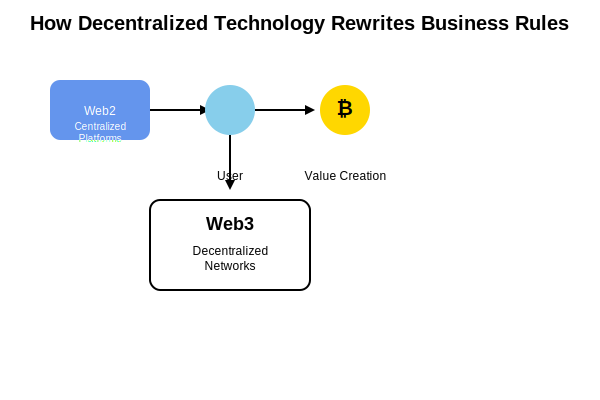
\includegraphics[keepaspectratio]{assets/images/ch2-overview.jpg}}

\section{數據主權革命}\label{ux6578ux64daux4e3bux6b0aux9769ux547d}

Web3技術引入了數據主權的可能性,從根本上改變了平臺和用戶之間的權力平衡。在當前系統中,每次點擊、購買、搜索和互動都會產生流向平臺所有者的數據,他們使用這些信息來優化自己的收入生成。用戶無法了解他們的數據如何被收集、處理或貨幣化,也沒有收到他們的活動創造的價值的補償。

去中心化身份系統使個人能夠跨多個平臺和應用程序擁有和控制他們的數字身份。用戶不再為每項服務創建單獨帳戶並向每個平臺交出個人信息,而是可以維護他們完全控制的便攜式身份。這種轉變對數字商業如何運作具有深遠影響,因為它消除了平臺通過數據鎖定效應困住用戶的能力。

當用戶擁有他們的數據時,他們可以選擇與不同服務分享哪些信息以及在什麼條件下分享。他們可以授予可以隨時撤銷的臨時訪問權限。最重要的是,他們可以就分享有價值的數據或參與數據生成活動進行補償談判。這為數據交換創造了市場機制,而不是當前的無補償提取系統。

這種影響延伸到商業環境中的客戶關係。通過Web3系統與客戶互動的商家可以在沒有中介平臺控制訪問的情況下發展直接關係。客戶數據仍然屬於客戶,他們可以選擇直接與他們信任的商家分享購買歷史、偏好和其他有價值的信息。這使得企業和客戶之間建立更真實的關係成為可能,同時無需對這些互動徵收平臺稅。

去中心化存儲系統確保用戶數據不會被平臺所有者丟失、損壞或操縱。存儲在分布式網路上的信息對用戶保持可訪問,無論任何特定平臺或服務提供商發生什麼。這創造了真正的數據可移植性,使用戶能夠在服務之間移動,同時保持其數字歷史和關係。

數據主權革命還通過用戶參與實現新形式的價值創造。當用戶擁有他們的數據和互動時,他們可以選擇直接將這些資產貨幣化,而不是允許平臺捕獲所有價值。這可能涉及向研究人員出售數據、參與產生直接收入的內容創作,或為創造代幣化獎勵的網路效應做出貢獻。

\section{從消費者到利益相關者}\label{ux5f9eux6d88ux8cbbux8005ux5230ux5229ux76caux76f8ux95dcux8005}

傳統平臺關係將用戶定位為購買產品或服務以換取金錢的消費者,或作為提供材料以換取平臺中介收入分享的內容創作者。Web3系統實現了基本角色轉換,用戶成為在他們幫助創建和維護的平臺和網路中擁有所有權利益的利益相關者。

這種轉換通過基於代幣的所有權系統發生,該系統根據網路參與者對網路價值的貢獻,在他們之間分配經濟權利。參與者不再為捕獲用戶活動大部分價值的平臺工作,而是可以在他們幫助建設和維護的網路中獲得所有權股份。這些所有權股份通常採用治理代幣的形式,提供網路決策的投票權,以及使持有者有權獲得網路收入份額的經濟代幣。

利益相關者模式以平臺系統無法實現的方式在平臺和參與者之間調整激勵。當用戶擁有他們參與的網路的一部分時,他們直接從網路增長和成功中受益。這為用戶貢獻高質量內容、提供有用反饋、招募新參與者以及以其他方式支持網路發展創造了強大的激勵。結果通常是比中心化平臺通過純粹提取關係能夠實現的更快增長和更高質量的結果。

與利益相關者地位相關的治理權利使得真正的民主參與平臺發展和政策決定成為可能。利益相關者不再接受平臺所有者決定實施的任何變化,而是可以提出修改、對重要決定進行投票,並集體指導網路演進。這創造了保持響應參與者需求而不是僅為所有者利益優化的系統。

利益相關者參與的經濟影響隨著成功網路增長而隨時間複合。幫助建立和發展網路的早期參與者可以看到其所有權股份的實質性升值,因為網路實現規模和採用。這為長期承諾和高質量參與創造了激勵,而不是許多平臺關係特徵的短期提取。

此外,利益相關者模式使風險分擔和網路發展中的協作投資成為可能。當參與者擁有所有權股份時,他們願意在網路改進中投資時間、金錢和努力,因為他們將分享這些投資的收益。與只有平臺所有者從網路改進中受益的系統相比,這可以加速創新和發展。

\section{智能合約商業}\label{ux667aux80fdux5408ux7d04ux5546ux696d}

智能合約代表Web3技術中最重要的創新之一,使協議的自動執行成為可能,而無需可信的中介。在商業環境中,智能合約可以自動化支付處理、執行服務協議、分配收入份額,並以數學精度和完全透明度管理複雜的多方交易。

通過智能合約自動化消除中介降低了交易成本,同時提高了執行的可靠性和速度。傳統商業交易通常需要銀行、支付處理器、託管服務和其他中介來確保所有方履行其義務。每個中介都為交易過程增加成本、複雜性和潛在故障點。智能合約可以用自動代碼替換許多這些中介,當滿足指定條件時,自動代碼執行預定義的邏輯。

考慮涉及商家、客戶、支付處理器和運輸公司的典型電子商務交易。傳統系統需要多個中介來協調這些互動,每個都收取費用並引入延遲。智能合約系統可以在貨物交付時自動處理付款,向商家和運輸公司分配適當的部分,處理稅收計算,並在出現問題時觸發客戶服務流程。整個交易根據預定義的規則執行,無需人工干預或中介協調。

智能合約還使通過傳統系統管理起來不切實際的更複雜商業安排成為可能。多方之間的收入分享協議可以自動化,以確保根據複雜公式準確及時地分配資金。訂閱服務可以根據使用模式或市場條件自動調整定價。當觸發事件發生時,保險索賠可以自動處理。這些能力使新的商業模式成為可能,這些模式以前太複雜或太昂貴而無法實施。

智能合約系統的透明度通過使所有交易邏輯可見和可驗證,在商業夥伴之間建立信任。參與者可以檢查管理其互動的代碼,確保自動化系統將按預期運行。這種透明度減少了爭議,並使可能不會相互信任履行複雜協議的各方之間的合作成為可能。

智能合約還使可編程貨幣成為可能,可以自動執行支出規則、儲蓄目標和投資策略。個人不再依賴個人紀律或第三方金融服務,而是可以創建自動化系統,根據預定規則分配收入,投資多元化投資組合,並執行複雜的金融策略,而無需持續的手動管理。

\section{中介的消亡}\label{ux4e2dux4ecbux7684ux6d88ux4ea1}

Web3技術使直接的點對點交易成為可能,消除了許多傳統中介角色,同時通過網路參與創造新形式的價值創造。參與者不再向中介支付費用來促進交易,而是可以直接互動,同時為服務其集體利益的共享基礎設施做出貢獻。

去中心化金融協議展示了中介消除在實踐中如何運作。傳統銀行要求客戶將錢存入金融機構,然後將這些資金借給借款人,同時捕獲利率差價。DeFi協議使存款人能夠通過自動化系統直接借給借款人,通常獲得更高的回報,而借款人支付更低的利率。中介利潤被消除,儲蓄在貸款人和借款人之間分享。

類似的動態適用於許多其他商業部門。內容創作者可以通過去中心化平臺直接向觀眾分發他們的作品,保留更大部分的收入,否則這些收入將流向平臺中介。自由職業者可以通過收取與傳統自由職業平臺相比微不足道費用的點對點網路與客戶聯繫。商家可以通過收取比中心化平臺更少佣金的去中心化市場直接向消費者銷售。

中介的消除並不意味著消除中介傳統提供的有價值服務。相反,這些服務在網路參與者之間分布或通過智能合約自動化。質量保證、爭議解決、支付處理和其他中介功能繼續存在,但通過去中心化機制而不是中心化中介提供。

這種轉換為個人創造了通過在去中心化網路內提供特定服務而不是為中介公司工作來賺取收入的機會。網路參與者可以通過內容審核、爭議解決、質量驗證、客戶服務和許多其他以前由平臺員工執行的功能獲得獎勵。這為個人創造了更靈活且通常更有利可圖的機會,同時降低了與中心化中介組織相關的開銷成本。

傳統中介的消亡還使生產者和消費者之間更直接的關係成為可能,導致更好的價格發現和更高效的市場。當移除多層中介時,生產者和消費者都可以通過其互動捕獲創造價值的更大部分。這通常導致消費者價格更低,生產者收入更高,差異代表消除中介提取。

\section{對商業策略的影響}\label{ux5c0dux5546ux696dux7b56ux7565ux7684ux5f71ux97ff}

向Web3商業的過渡要求企業在客戶獲取、關係管理和價值創造方面採取根本性改變。理解並適應這些變化的公司將發現顯著的競爭優勢,而那些堅持依賴平臺策略的公司可能發現自己越來越處於劣勢。

Web3環境中的客戶獲取專注於提供真正價值和建立信任,而不是通過廣告平臺購買注意力。由於Web3用戶擁有他們的數據和身份,他們可以更容易地評估和比較不同選項。企業必須基於提供的實際價值而不是營銷複雜性或廣告支出能力進行競爭。

關係管理從平臺中介的互動轉向與擁有其數據和身份的客戶的直接參與。這使得更深入、更真實的關係成為可能,但要求企業提供持續價值,而不是依賴平臺鎖定效應來維持客戶忠誠度。在為客戶創造真正價值方面表現出色的公司將蓬勃發展,而那些依賴信息不對稱或轉換成本的公司將面臨困難。

在Web3環境中,價值創造機會顯著擴大,因為企業可以參與網路效應和代幣經濟,而不是簡單地從交易中提取利潤。公司可以創建並參與隨著吸引更多參與者而增長價值的去中心化網路。這可以提供通過傳統商業模式無法獲得的指數增長機會。

Web3轉型既代表技術轉變,也代表向更公平、更高效的數字商業形式的哲學演進。正如我們將在第三章中探討的,這些原則的實際實施需要平臺設計、代幣經濟學和社區治理的系統方法。鏈上商業的六大支柱提供了一個框架,用於理解這些抽象概念如何轉化為能夠大規模運營同時保持去中心化和參與者所有權好處的具體商業系統。

\chapter{鏈上商業的六大支柱}\label{sec-six-pillars}

去中心化商業的架構基礎

從傳統平臺式商業向去中心化鏈上商業的轉變不僅需要技術創新。它需要一個全面的框架來解決信任、價值分配、可擴展性和可持續增長的根本挑戰,這些挑戰限制了以往創建公平數位經濟的嘗試。鏈上商業的六大支柱提供了這個框架,為構建能夠大規模運營同時保持去中心化和參與者所有權好處的商業系統提供系統性方法。

這些支柱作為一個集成系統而不是獨立組件共同工作。每個支柱解決傳統商業系統中的特定弱點,同時加強其他支柱以創建穩定、自我維持的經濟生態系統。支柱之間的相互依賴確保鏈上商業系統既能實現實際採用所需的效率,又能實現長期參與者承諾所必需的公平性。

理解這些支柱需要檢查它們的個體功能和在完整鏈上商業實施中的集體運作。正如我們在第1章和第2章中探討的,向基於流通的財富創造的轉變和Web3對傳統平臺模式的顛覆為商業組織的新方法創造了機會。六大支柱提供了在實踐中實現這些機會的具體機制。

\begin{figure}[H]

{\centering \pandocbounded{\includegraphics[keepaspectratio]{assets/images/Ch3-6-pillars.jpg}}

}

\caption{六大支柱}

\end{figure}%

\section{支柱一:公平利潤分享機制}\label{ux652fux67f1ux4e00ux516cux5e73ux5229ux6f64ux5206ux4eabux6a5fux5236}

傳統商業系統將利潤集中在平臺所有者和投資者中,而僅向通過其活動實際創造價值的參與者分配工資或小額佣金。鏈上商業系統通過實施自動利潤分享機制逆轉這種動態,該機制根據所有貢獻者對網路成功的實際貢獻在他們之間分配價值。

公平利潤分享通過智能合約運作,根據預定義公式在不同參與者之間自動分配交易收入的部分。當客戶通過鏈上商業系統進行購買時,交易價值流經自動分配機制,立即將適當部分分配給商家、客戶、推薦合作夥伴、網路基礎設施提供商和對交易成功的其他貢獻者。

自動化消除了表徵傳統利潤分享安排的爭議和延遲。參與者在交易完成後立即收到其分配部分,所有計算根據公開可審計的智能合約代碼透明執行。這通過數學確定性而不是依賴機構承諾或法律執行機制創造信任。

具體分配公式可以針對不同類型的企業和市場進行定製,同時保持公平和透明的核心原則。典型分配可能將60\%的交易價值分配給客戶作為獎勵,15\%分配給商家作為激勵補償,4\%分配給推薦合作夥伴,3\%分配給區域協調員,18\%根據各種網路參與者對交易促進的貢獻在他們之間分配。

這些百分比代表的不僅僅是簡單的收入分享。它們構成了商業價值如何創造和分配的根本重構。鏈上商業系統不是從參與者那裡提取價值以最大化平臺利潤,而是優化參與者成功和網路增長。這創造了正回饋循環,其中成功的參與者吸引更多活動到網路,為所有參與者產生增加的價值。

利潤分享機制還超越個人交易,涵蓋網路增長和發展。對網路擴張、品質改進或基礎設施發展做出貢獻的參與者從其貢獻創造的增加價值中獲得持續補償。這以傳統就業或承包商關係無法實現的方式將個人激勵與集體網路成功對齊。

此外,自動化利潤分享的透明性質使參與者能夠準確理解其補償如何計算,並驗證他們獲得公平待遇。這種透明度減少衝突並在可能對收入分享聲明持懷疑態度的參與者之間建立信任。

\section{支柱二:💡 穩定的通證價值支撐模型:AC
的底層邏輯}\label{ux652fux67f1ux4e8c-ux7a69ux5b9aux7684ux901aux8b49ux50f9ux503cux652fux6490ux6a21ux578bac-ux7684ux5e95ux5c64ux908fux8f2f}

🔄 \textbf{以真實交易為基礎的價值支撐}\\
● F2C
系統中的每一筆交易,都包含F2C平臺設定的「讓利金額」,這部分讓利即成為 AC
的「發行依據」,也就是說:\\
AC 不是空發,而是因價值創造而生。

●
F2C平臺設定的「讓利金額」以USDC的形式,自動注入「價值底池」(底層資金池),形成鏈上流動性支撐,並為
AC 提供穩定的價格錨點。

⚙️ \textbf{由市場動態自動調整釋放比例}\\
AC 的釋放與回收,並非固定比例,而是根據以下幾項核心指標動態調控:\\
● F2C 平臺整體交易額\\
● 市場活躍度(用戶數與頻率)\\
● 當前市場購買力(對 AC 的實際需求)

透過這種機制,AC
可避免過度通縮或通膨問題,即使面對外部波動,也能保持價值穩定性與韌性。

🧱 \textbf{三重價值基礎:現金流 + 使用場景 + 信任證明}\\
1. 現金流支持:每一枚 AC 背後都有實際的商業消費行為\\
2. 實際應用場景:可用於折抵費用、進行治理、參與獎勵等\\
3. 信任證明機制:所有 AC 發行都源自可驗證的鏈上活動與真實價值

與傳統依賴炒作或二級市場拉盤的模型不同,AC
建立的是一個真實經濟循環,能夠長期持續運作,不依賴資金盤式的假象繁榮。

🔁 \textbf{二級市場的作用:放大,而非製造價值}\\
雖然 AC
本身的價值建立於使用場景與交易行為,但二級市場的活躍仍然具有關鍵性意義:\\
● 為持有者提供流動性出場的管道\\
● 反映市場對平臺與生態的信心與預期\\
● 對長期參與者與貢獻者提供資本增值可能性

簡而言之,二級市場是價值的鏡子,而非來源,它能放大價值,而不是憑空創造價值

\section{支柱三:可擴展的商家成長階梯}\label{ux652fux67f1ux4e09ux53efux64f4ux5c55ux7684ux5546ux5bb6ux6210ux9577ux968eux68af}

鏈上商業系統必須容納從個人企業家到大型既定企業的參與者,同時提供既有利於個體商家又有利於更廣泛網路的增長和發展路徑。可擴展的商家成長階梯創造結構化進步機會,鼓勵參與和投資,同時保持網路凝聚力和共享價值觀。

基礎級別以最小進入障礙歡迎個人企業家和小企業。新商家可以加入鏈上商業網路而無需重大前期投資或複雜資格程序。他們立即獲得基於代幣的獎勵系統、自動化支付處理和幫助他們在網路生態系統內建立業務的基本營銷工具。

隨著商家實現與交易量、客戶滿意度和網路貢獻相關的特定里程碑,他們解鎖對增強功能和好處的訪問。增長階梯可能包括訪問高級分析工具、優先客戶服務、擴展的代幣分配百分比,以及與網路內其他成功商家的協作機會。

區域合作夥伴關係機會代表商家發展的下一個級別,使成功的個體商家能夠與其地理區域的其他商家協調,創建本地商業生態系統。區域合作夥伴可以匯集資源進行營銷活動,分享客戶群,並開發互補服務產品,為本地客戶增加價值,同時加強其市場中的整體網路存在。

商家參與的最高級別涉及與核心網路開發團隊的戰略合作夥伴關係,使大型商家能夠影響網路方向和發展優先級,同時承擔網路增長和穩定的更大責任。這些戰略合作夥伴可能運營多個地點,指導新商家,或提供有利於整個網路生態系統的專業服務。

階梯結構為長期參與和對網路成功的投資創造明確激勵。商家理解他們在網路內的增長取決於為客戶提供真正價值和積極促進網路發展。這以傳統業務發展計劃經常無法實現的方式將個人成功與集體網路繁榮對齊。

增長階梯的每個級別提供有意義的好處,證明與晉升相關的增加承諾和責任的合理性。從個人企業家到區域合作夥伴到戰略聯盟的進展創造了職業發展路徑,可以容納終身商業增長,同時保持與鏈上商業網路的聯繫。

可擴展結構還確保網路治理對不同商業規模和發展階段的參與者需求保持響應。個人企業家通過民主治理機制在網路決策中有發言權,而更大的戰略合作夥伴為網路發展和擴張提供穩定性和資源。

\section{支柱四:高信任社區網路}\label{ux652fux67f1ux56dbux9ad8ux4fe1ux4efbux793eux5340ux7db2ux8def}

傳統多層次營銷和金字塔計劃創建膚淺的社區結構,最終優先考慮招募和層級而不是真正的價值創造和相互支持。鏈上商業網路基於共享成功、透明運營和協作價值創造而不是提取和剝削建立真實的社區關係。

高信任社區網路的基礎在於消除在傳統系統中創造剝削的結構性激勵。鏈上商業參與者不主要從招募新成員或建立下線組織中獲利。相反,他們的成功取決於通過商家服務、客戶滿意度和有利於所有參與者的網路發展活動促進真正的價值創造。

網路透明度創造防止剝削關係發展的問責機制。所有交易、獎勵分配和治理決策都記錄在區塊鏈系統上,使任何參與者能夠驗證公平待遇和適當補償。這種透明度消除了在傳統層級系統中實現操縱和剝削的資訊不對稱。

社區網路結構強調水準協作而不是垂直層級。網路參與相似級別的參與者共同解決問題、分享資源和開發新機會,而不是在組織層級中為有限職位相互競爭。這種協作方法創造更強的關係和更可持續的社區紐帶。

區域集群實現本地社區發展,同時保持與更廣泛全球網路的聯繫。特定地理區域的參與者可以發展個人關係,協調本地營銷努力,並提供相互支持,同時從通過更大網路可獲得的資源和機會中受益。本地社區和全球網路訪問之間的平衡提供個人聯繫和可擴展機會。

教育和支持系統確保所有社區成員獲得網路內成功所必需的知識和資源。成功參與者不是囤積資訊以維持競爭優勢,而是被激勵分享知識和提供指導,因為網路增長通過增加活動和代幣價值升值使每個人受益。

衝突解決機制使社區成員能夠通過透明、公平的過程而不是依賴權威人物的任意決定解決爭議和分歧。去中心化治理系統提供維持社區凝聚力同時保護個人權利和利益的結構化問題解決方法。

高信任社區網路還創造社會驗證和支持系統,幫助參與者在挑戰期間保持動機和承諾。財務激勵和社會關係的結合創造比純粹經濟安排能夠實現的更強參與者保留。

\section{支柱五:真正的共用收入設計}\label{ux652fux67f1ux4e94ux771fux6b63ux7684ux5171ux7528ux6536ux5165ux8a2dux8a08}

大多數傳統收入分享計劃提供不代表真正利潤參與的代幣金額或條件性好處。鏈上商業系統實施真正的共用收入設計,參與者獲得實際網路利潤的有意義部分,而不是名義獎勵或有限折扣計劃。

真正的共用收入通過數學公式運作,該公式根據不同類別參與者對網路成功的貢獻在他們之間分配網路收入的特定百分比。這些分配代表真實經濟價值而不是促銷噱頭或營銷費用。參與者理解他們的補償來自真正的利潤分享而不是新參與者招募或其他不可持續來源。

收入分享超越即時交易獎勵,涵蓋持續的網路盈利能力。隨著鏈上商業網路增長並產生增加的交易量,所有參與者通過增加的收入分享而不是讓增長好處被平臺所有者或早期投資者獨佔而從這種增長中受益。

網路參與者通過多種類型的貢獻而不是單一活動獲得收入分享。客戶推薦、商家支持、內容創建、網路治理參與和基礎設施發展都可以基於其對網路成功的實際價值貢獻產生收入分享。這種價值創造機會的多樣性確保具有不同技能和興趣的參與者可以找到有意義的貢獻和受益方式。

共用收入設計還包括通過代幣所有權的升值機會。隨著網路增長並變得更有價值,擁有AC代幣的參與者除了持續收入分享外還從價值升值中受益。這為活躍網路參與者創造即時收入機會和長期財富建設可能性。

收入計算和分配的透明度確保參與者可以驗證其公平待遇並理解其貢獻如何轉化為補償。定期報告和可審計智能合約系統提供網路財務績效和收入分配的可見性,建立信任並使參與者能夠就其網路參與水準做出明智決策。

收入分享公式可以通過民主治理過程隨時間演變,確保隨著網路條件變化,補償結構保持公平和競爭力。參與者在收入分配優先級決策中有發言權,可以提議更好服務網路發展和參與者利益的修改。

\section{支柱六:高頻次使用場景}\label{ux652fux67f1ux516dux9ad8ux983bux6b21ux4f7fux7528ux5834ux666f}

成功的鏈上商業網路必須服務具有高頻次使用場景的真實商業需求,而不是依賴投機交易或缺乏實用效用的新穎應用。第六支柱確保網路活動由真正的經濟需求而不是人工採用激勵或投機投資驅動。

高頻次使用場景涉及滿足參與者日常需求的商品和服務,創造定期、可預測的網路活動模式。這些可能包括雜貨購物、餐飲、交通、娛樂、個人服務和其他人們定期消費的商品類別。通過專注於必需品和頻繁購買的商品,鏈上商業網路建立可持續的使用模式,支持長期增長和穩定。

必需品焦點確保網路活動保持對客戶有價值和相關,而不管更廣泛的經濟條件或加密貨幣市場趨勢如何。人們將繼續需要食物、住房、交通和其他基本服務,為網路活動提供穩定基礎,不受投機興趣波動的影響。

地理密度創造網路效應,增加對參與者的便利性和價值,同時減少與線上交易相關的運輸成本和交付時間。當本地區域有足夠數量的參與商家時,客戶可以將AC代幣用於其大部分日常購買,增加代幣實用性並減少轉換回傳統貨幣的需要。

社區整合將鏈上商業網路嵌入本地經濟和社會結構中,創造超越純財務激勵的參與動機。當網路成為社區生活的重要組成部分時,參與者開發維持和支持網路成功的社會和經濟利益。

商家多樣性確保參與者可以將AC代幣用於廣泛的商品和服務,增加代幣在日常生活中的實用性。全面的商家生態系統減少參與者需要轉換回傳統貨幣進行購買的頻率,增加網路內的價值流通並減少外部依賴。

品質標準維持客戶滿意度和網路聲譽,確保高頻次使用產生積極體驗,鼓勵持續參與。網路必須平衡增長與品質控制,確保擴張不會以可能破壞長期成功的客戶體驗為代價。

服務整合創造全面生活方式解決方案,參與者可以通過單一網路訪問其大部分需求。這可能包括與本地服務提供商的夥伴關係,如醫療保健提供者、教育機構、娛樂場所和專業服務,創造一個能夠支持參與者整個生活方式的綜合生態系統。

技術便利性確保高頻次使用保持方便和高效,無論對於精通技術還是不精通技術的參與者。使用者介面、支付處理和客戶服務系統必須支持快速、可靠的交易,不會在日常使用中造成摩擦或延遲。

六個支柱的相互作用創造了超過其組成部分總和的綜合系統。公平利潤分享激勵參與,而穩定代幣價值支撐建立信心。可擴展增長階梯提供發展機會,而高信任社區網路創造支持環境。真正共用收入設計確保參與者從網路成功中受益,而高頻次使用場景提供使整個系統實用和可持續的真實商業應用。

這種集成方法解決了阻礙以往創建公平去中心化經濟嘗試的根本挑戰。通過同時解決技術、經濟、社會和實用考慮,六支柱框架為構建真正服務參與者利益同時實現可持續增長和發展的鏈上商業系統提供全面基礎。

正如我們將在第4章中探討的,這些支柱在「花得越多,賺得越多」系統中發揮作用,創造正回饋循環,獎勵參與並推動網路擴張,同時保持使鏈上商業對所有參與者有價值和公平的核心原則。

\part{第二部分:轉型機制}

\chapter{``花得越多,賺得越多''運營系統}\label{sec-spend-earn-system}

消費如何在新經濟中成為投資

花錢實際上可以增加財富而不是減少財富這一概念,代表了鏈上商業系統最反直覺的方面之一。傳統經濟思維將消費和投資視為對立活動:用於商品和服務的錢不再可用於財富建設投資。鏈上商業通過創建消費活動同時為參與者生成投資回報的機制,從根本上重構了這種關係。

這種轉換通過複雜的代幣分配系統發生,該系統將消費者支出的一部分轉換為可交易的數字資產,同時保持表徵正常商業交易的基本價值交換。客戶收到他們購買的商品和服務,同時還收到代表在促成其購買的商業網路中的所有權股份的代幣。結果是一個系統,其中增加的參與和支出產生增加的財富積累,而不是耗盡財政資源。

理解這個系統如何運作需要檢查傳統消費支出轉換為投資資產的具體機制,確保可持續回報的數學基礎,以及使這樣的系統能夠創造真正價值而不是簡單地在參與者之間重新分配現有財富的經濟原則。

\section{交易到資產轉換}\label{ux4ea4ux6613ux5230ux8cc7ux7522ux8f49ux63db}

花得越多賺得越多系統的基礎機制在於將交易金額自動轉換為隨時間升值的代幣資產。當客戶通過鏈上商業平臺進行購買時,商家的利潤分享承諾立即轉換為Apollo
Coin(AC)代幣,根據預定分配公式分配給客戶和其他網路參與者。

這種轉換過程通過智能合約運作,智能合約自動執行複雜的計算和分配,而不需要人工干預或對第三方管理員的信任。商家設定利潤分享百分比,代表他們願意分配給網路代幣分配的總銷售額部分。這個百分比通常從交易價值的3\%到99\%不等,代表商家為了換取參與鏈上商業網路產生的營銷利益和客戶忠誠度而放棄的真實經濟價值。

考慮這種轉換在實踐中如何運作的具體例子。客戶在參與鏈上商業並承諾30\%利潤分享的餐廳購買50美元的餐食。客戶支付50美元並收到他們的餐食,完全如同任何傳統交易。然而,智能合約系統還自動將15美元(50美元的30\%)根據當前二級市場即時單價轉換為AC代幣,並根據網路的分配公式分配這些代幣。

使用第三章討論的分配模型,轉換金額的60\%將作為獎勵流向客戶,15\%作為參與激勵流向商家,4\%流向推薦商家的夥伴,3\%流向區域協調員,其餘18\%在各種網路基礎設施參與者之間分配。這意味著客戶將收到價值9美元的AC代幣,而商家收到價值2.25美元的代幣,儘管已經向轉換池貢獻了15美元的利潤率。

交易到資產轉換為客戶創造即時價值,同時建立通過增加的客戶忠誠度和重複業務使商家受益的長期關係。客戶產生返回參與商家的財務激勵,因為他們的支出通過代幣升值產生持續的投資回報。商家從降低的客戶獲取成本和增加的交易頻率中受益,通常超過分配給代幣分配的利潤率的補償。

轉換機制還創造了網路效應,隨著系統增長使所有參與者受益。每筆交易都加強了AC代幣的儲備支撐,同時展示了對網路服務的真實經濟需求。儲備加強和需求驗證的結合支持代幣價值升值,使整個網路中的所有代幣持有者受益。

此外,交易到資產轉換的自動性質消除了通常阻止消費者參與傳統投資計劃的複雜性和障礙。客戶不需要理解代幣機制、管理數字錢包或做出明確的投資決策。轉換作為正常購物活動的一部分無縫發生,使投資參與對可能永遠不會參與傳統加密貨幣或投資系統的個人可及。

\section{AC代幣經濟}\label{acux4ee3ux5e63ux7d93ux6fdf}

Apollo
Coin代幣經濟提供了使可持續花得越多賺得越多運營成為可能的數學基礎。與主要從交易活動和市場情緒獲得價值的投機性加密貨幣不同,AC代幣由通過實際商業交易產生的真實經濟儲備支撐。這種支撐創造了內在價值,支持基於基本經濟活動而不是投機泡沫的長期價格穩定和升值。

儲備支撐系統通過去中心化智能合約運作,自動將商家利潤分享貢獻的一部分存入儲備池。這些儲備以穩定的加密貨幣如USDC(美元幣)持有,與傳統貨幣保持可靠的價值關係。儲備池為AC代幣價值提供數學支持,同時使代幣持有者能夠在特定條件下將代幣兌換為基礎儲備資產。

流通的AC代幣和儲備支撐之間的關係創造了自然的價格穩定機制。當AC代幣交易低於其儲備支撐的內在價值時,出現購買被低估代幣並可能將其兌換為更高價值儲備資產的套利機會。相反,當代幣交易高於內在價值時,通過新商家交易的額外代幣創建增加供應,直到價格在數學支持水平附近穩定。

代幣經濟還包含鼓勵流通而不是囤積的速度激勵。在網路內用於購買的AC代幣比作為靜態投資持有時產生額外價值。積極與參與商家消費AC代幣的網路參與者通常收到獎金分配、推薦獎勵或其他激勵,與被動持有者相比增加他們的總代幣積累。

AC代幣分配基礎的數學模型確保網路增長創造正和結果而不是零和重新分配。隨著更多商家加入網路並向儲備池貢獻利潤分享,所有未償代幣的總支撐增加。同時,增加的商家參與為代幣利用創造更多機會,通過基本供需動態產生支持價格升值的需求。

地理擴張戰略通過創建支持代幣實用性和需求的多個區域市場進一步加強代幣經濟。當特定地理區域內的足夠商家參與網路時,客戶可以將AC代幣用於他們的許多日常購買,創造超越投機交易價值的實用性。這種基於實用性的需求為代幣價值提供可持續支持,獨立於加密貨幣市場波動。

儲備支撐和代幣分配的透明度創造了在系統長期可持續性中建立參與者信心的問責制。與依賴機構承諾或複雜金融工程的傳統投資計劃不同,AC代幣持有者可以通過基於區塊鏈的審計系統驗證其代幣持有和基礎儲備資產之間的數學關係。

\section{閉環價值系統}\label{ux9589ux74b0ux50f9ux503cux7cfbux7d71}

花得越多賺得越多系統最複雜的方面在於創建閉環價值系統,這些系統放大參與者的利益,同時減少對外部經濟條件的依賴。這些系統通過創建多個相互關聯的價值流來實現可持續性,這些價值流通過網路效應和參與者行為優化相互加強。

主要循環通過客戶支出、代幣積累和網路內再投資運作。通過購買收到AC代幣的客戶被激勵與其他網路商家消費這些代幣,既為了利用其代幣價值,又為了通過持續的網路參與產生額外的代幣獎勵。這創造了一個流通模式,其中代幣在客戶和商家之間流動,同時在每個交易點產生增量價值。

通過推薦和社區建設活動出現次級循環,這些活動擴展網路參與並增加總交易量。成功為網路招募新商家或客戶的參與者從其推薦產生的增加活動中獲得持續補償。這為網路傳播和增長創造激勵,通過增加代幣實用性和升值而不是簡單地在更多參與者之間稀釋現有價值來使現有參與者受益。

商家生態系統通過協作和交叉推薦活動創造額外的價值循環。參與的商家經常發展互補關係,他們為其專業之外的服務相互推薦客戶。餐廳可能與附近的水療中心、零售店或娛樂場所合作,創建全面的本地網路,增加客戶便利性,同時為參與企業產生推薦收入。

區域協調機制使本地商家網路能夠匯集資源用於營銷活動、客戶獲取計劃和基礎設施開發,使所有網路參與者受益。這些協作投資產生根據其貢獻水平和網路活動在參與商家之間分配的回報,為集體而不是純粹個人優化創造激勵。

閉環系統還包含基於參與者行為和結果優化網路性能的反饋機制。分析系統跟踪客戶滿意度、商家盈利能力、代幣流通模式和網路增長指標,以識別優化機會並調整系統參數以改善性能。這種持續改進過程確保網路演進以更好地服務參與者需求,同時保持數學可持續性。

質量保證循環通過監控商家績效和客戶滿意度水平來維護網路完整性。始終提供積極客戶體驗的商家獲得增強的利益和促銷支持,而那些產生投訴或負面反饋的商家可能面臨減少的參與利益或從網路中移除。這為保護網路聲譽和客戶保留的服務質量創造激勵。

多個價值循環的整合創造了抵禦外部經濟破壞的韌性。當傳統經濟條件惡化時,閉環網路可以通過內部流通和交換活動繼續為參與者創造價值。這種韌性在經濟不確定性期間變得特別有價值,當傳統投資和就業機會可能變得不太可靠時。

\section{風險緩解和系統保障}\label{ux98a8ux96aaux7de9ux89e3ux548cux7cfbux7d71ux4fddux969c}

花得越多賺得越多模式包含全面的風險緩解策略,將其與賭博、投機或不可持續的金融計劃區別開來。這些保障保護參與者投資,同時通過保守的數學模型和透明的操作程序確保系統可持續性。

儲備支撐要求確保代幣價值由真實經濟資產而不是投機市場情緒支撐。相對於未償代幣的儲備支撐百分比通過算法控制維持,防止相對於可用儲備資金的代幣過度發行。這為代幣價值創造數學底限,保護參與者免受表徵純粹投機投資的全部損失情況。

商家審查程序在企業能夠參與利潤分享計劃之前驗證其合法性和可持續性。新商家必須展示穩定的業務運營、適當的許可和註冊,以及足夠的交易量來支持其提議的利潤分享承諾。這種篩選過程減少了可能損害網路完整性的欺詐或不可持續商家參與的風險。

地理多元化將網路風險分散到多個區域市場和經濟條件中。鏈上商業網路不是將所有活動集中在單一地點或行業,而是故意在地理區域和商業部門中培養商家多樣性。這種多元化減少了地方經濟破壞對整體網路穩定性和參與者回報的影響。

治理機制使參與者能夠輸入系統修改和風險管理政策。代幣持有者可以提議並投票表決儲備要求、分配公式、商家資格標準和影響網路運營和參與者安全的其他系統參數的變化。這種民主治理確保風險管理政策反映參與者偏好和不斷變化的市場條件。

法規合規程序確保網路運營符合適用的金融法規和消費者保護法。管理證券、支付處理、消費者保護和稅收的法律框架被仔細分析並納入系統設計,以防止可能威脅網路運營或參與者利益的法規衝突。

退出機制使參與者能夠在各種情況下收回其投資。代幣贖回選擇、商家退出程序和客戶退款政策為參與者在其情況或偏好發生變化時退出網路提供多種途徑。這些退出選擇通過有序的離開程序減少參與者風險,同時維護網路完整性。

\section{投資回報分析}\label{ux6295ux8cc7ux56deux5831ux5206ux6790}

花得越多賺得越多系統的數學基礎使得能夠在各種情景和市場條件下對參與者回報進行定量分析。這些計算展示了普通支出活動如何產生類似投資的回報,同時保持正常商業交易的實用效用。

複合增長組件來自在網路內再投資代幣以產生額外代幣積累。使用其AC代幣進行後續購買的客戶繼續賺取額外代幣,同時從其現有代幣持有的任何升值中受益。這種複合效應可以隨時間顯著放大總回報,特別是對於保持高水平網路參與的參與者。

區域網路效應通過跨商家利用和推薦計劃創造額外的回報機會。成熟區域網路中的參與者在結合即時代幣分配、升值收益、推薦收入和網路參與獎勵時,經常報告超過其支出活動200\%的總年回報。這些回報反映了當足夠的商家和客戶參與本地化鏈上商業生態系統時出現的網路效應。

風險調整回報計算考慮了潛在的代幣價值波動和網路採用不確定性。即使在假設適度網路增長和有限代幣升值的保守情景下,參與者通常實現超過傳統儲蓄賬戶、貨幣市場基金和許多傳統投資選擇的正回報。即時代幣分配和適度升值的結合通常產生從純財務角度證明參與合理的回報。

增加購買力的實際好處通過改善網路商家社區內商品和服務的獲取進一步增強有效回報。參與者經常發現新業務,從網路商家獲得優惠待遇,並獲得提供超越純財務回報價值的獨家優惠和服務。這些定性好處補充定量回報,創造證明網路參與合理的綜合價值主張。

長期財富建設潛力來自在多年期間持續參與不斷增長的鏈上商業網路。在擴展網路中保持一致參與和再投資的參與者經常積累隨著網路實現區域或國家規模而顯著升值的大量代幣持有。這種財富建設潛力將日常支出活動轉化為可以產生實質性長期財務好處的系統投資計劃。

花得越多賺得越多運營系統代表了消費者經濟學的基本創新,將個人支出決策與投資回報結合,同時支持真正的業務發展和社區繁榮。正如我們將在第五章中探討的,這個系統與傳統的多級營銷、電子商務和特許經營模式截然不同,這些模式經常在個人和集體利益之間創造衝突。鏈上商業的數學基礎和系統保障創造可持續的價值生成,使所有參與者受益,同時服務於本地和區域市場的真實經濟需求。

\chapter{超越傳銷、電商和特許經營}\label{sec-beyond-traditional}

與傳統商業模式的根本差異

鏈上商業系統經常被誤解為多級營銷、電子商務平臺或特許經營運營的變體,因為它們與這些傳統商業模式共享某些表面特徵。所有這些都涉及參與者網路、多方之間的收入分享,以及通過參與者招募和保留實現增長。然而,鏈上商業的基本結構、激勵系統和價值創造機制與這些傳統方法截然不同,以解決限制其可持續性和公平性的系統性問題的方式。

理解這些差異需要檢查的不僅是每種模式的操作機制,還有決定其長期可行性和對參與者影響的基礎經濟原理和激勵結構。雖然傳統模式經常在個人成功和集體可持續性之間創造衝突,但鏈上商業通過精心設計的代幣經濟學和治理機制調整個人和集體利益。

這種區別很重要,因為許多有前途的商業創新由於建立在從傳統模式借用的有缺陷的基礎假設上而失敗。鏈上商業代表了一種真正新的商業組織方法,超越現有框架的限制,同時保留其有益元素。

\section{傳銷陷阱:多級營銷的結構缺陷}\label{ux50b3ux92b7ux9677ux9631ux591aux7d1aux71dfux92b7ux7684ux7d50ux69cbux7f3aux9677}

多級營銷系統創造分布式機會的外觀,同時實際上以後期加入者為代價,在早期參與者中集中財富和權力。MLM系統的數學結構確保絕大多數參與者將虧損,而一小部分實現實質性回報,創造不可避免地導致系統崩潰的不可持續動態。

MLM系統的根本缺陷在於它們依賴指數招募增長來為現有參與者產生收入。每個參與者必須招募多個新參與者,每個新參與者必須招募額外的參與者來維持收入水平。這創造了金字塔結構,其中早期參與者從越來越多的後期參與者的努力中受益,而沒有提供相稱的回報價值。

考慮典型MLM結構的數學,其中每個參與者需要招募五個新參與者才能實現有意義的收入。在五個層級的招募後,系統需要超過三千名參與者在底層支持大約六百名更高層級的參與者。在十個層級後,底層需要數百萬參與者,迅速超過大多數市場的可用人口。這種數學不可能性保證大多數參與者將失敗實現有意義的回報,無論他們的努力或技能如何。

MLM系統還創造優先考慮招募而不是實際價值創造的不當激勵。參與者通過招募新分銷商比通過向最終客戶銷售產品賺更多錢,導致專注於銷售演示和招募活動而不是客戶服務和產品改進。這種不匹配經常導致糟糕的客戶體驗和無法在正常市場條件下有效競爭的低質量產品。

MLM系統中常見的庫存裝載要求迫使參與者購買他們無法銷售的產品,通過對未來招募成功的承諾來證明即時財務損失的合理性,創造即時財務損失。這些庫存要求為MLM公司產生收入,同時將財務風險轉移給必須在獲得任何回報之前投資自己資金的參與者。

鏈上商業通過基於實際交易價值而不是招募活動的獎勵來消除這些結構問題。參與者從真正的商業交易中獲得代幣,其中客戶購買他們實際想要的商品和服務,而不是從向新招募者銷售商業機會中獲得。沒有人需要購買庫存或維持最低購買量來參與系統。

代幣分配機制確保價值根據參與者對網路活動的貢獻流向所有參與者,而不是他們在招募層級中的位置。與只有頂級參與者實現實質性回報的MLM系統不同,鏈上商業可以為所有參與者提供有意義的好處,因為獎勵來自共享的經濟價值創造,而不是從較低層級到較高層級的重新分配。

此外,鏈上商業系統隨著增長變得更有價值,創造正和結果,其中網路擴張使現有參與者受益,而不是稀釋他們的回報。MLM系統隨著增長變得不太可持續,因為招募要求變得越來越難以實現,而鏈上商業系統隨著更多商家和客戶參與變得更有用和有價值。

\section{平臺監獄:電子商務依賴和剝削}\label{ux5e73ux81faux76e3ux7344ux96fbux5b50ux5546ux52d9ux4f9dux8cf4ux548cux525dux524a}

現代電子商務平臺創建了從商家提取價值的複雜系統,同時使他們依賴平臺服務來獲得市場准入。亞馬遜、eBay、Shopify和類似平臺最初通過以合理成本提供有價值的服務來吸引商家,但隨著商家變得依賴平臺流量生存,逐漸增加費用和限制。

平臺監獄通過多個相互關聯的機制運作,使離開隨時間變得越來越昂貴和困難。商家在建立其平臺存在、積累客戶評論、為平臺算法優化以及將其運營與平臺工具集成方面投資大量精力。如果商家試圖離開平臺,這些投資成為擱淺成本,創造轉換成本,使平臺能夠逐漸增加其提取而不失去商家參與。

客戶關係控制代表平臺對商家控制的最重要元素。平臺擁有所有客戶數據和關係,防止商家與其買家建立直接聯繫。商家無法在平臺外聯繫客戶,無法將客戶列表轉移到替代平臺,無法建立超越平臺依賴的品牌忠誠度。這種客戶關係控制確保商家保持依賴平臺服務,無論這些服務如何演變。

商家可見性的算法操縱創造了平臺通過廣告和優質放置服務貨幣化的人為稀缺性。以前收到有機流量的商家發現他們的可見性降低,除非他們從平臺購買廣告或優質服務。這迫使商家為訪問他們以前通過有機發現到達的客戶付費,逐漸將平臺好處轉換為平臺成本。

費用升級發生在平臺實現市場主導地位和商家變得依賴平臺流量時。當平臺提供真正價值時看起來合理的初始費用隨著平臺優化最大收入提取而逐漸增加。圍繞平臺經濟建立業務的商家發現自己被困在不可持續的費用結構和無法通過替代渠道替換平臺流量之間。

鏈上商業通過為商家提供通過基於代幣的忠誠度系統與客戶的直接關係來解決這些問題。從商家購買收到AC代幣的客戶與這些商家發展獨立於任何平臺中介存在的直接財務關係。商家可以與客戶溝通,建立直接關係,並通過代幣獎勵而不是依賴平臺算法和廣告系統來維持客戶忠誠度。

鏈上商業的去中心化性質防止任何單一實體控制商家對客戶的訪問或為了利潤操縱商家可見性。網路治理機制使商家能夠參與網路發展和政策變化的決定,確保網路演進服務商家利益而不是平臺所有者利潤最大化。

基於代幣的客戶獲取創造隨時間升值而不是變得更昂貴的可持續客戶關係。隨著鏈上商業網路增長和代幣價值升值,現有客戶關係變得更有價值,而不是需要增加廣告支出來維持。這創造了獎勵商家提供優秀客戶服務而不是通過增加平臺費用懲罰他們的正反饋循環。

\section{特許經營限制:運營和地理}\label{ux7279ux8a31ux7d93ux71dfux9650ux5236ux904bux71dfux548cux5730ux7406}

傳統特許經營系統提供商業模式複製和品牌識別,以換取大量前期投資、持續的特許權使用費支付和限制特許經營者靈活性和增長潛力的運營限制。雖然特許經營可以提供經過驗證的商業模式和營銷支持,但它也創造了阻止特許經營者適應當地市場條件或追求創新機會的依賴性和限制。

特許經營費用結構將成本和風險前置到特許經營者身上,同時確保特許經營商的收入,無論特許經營者是否成功。初始特許經營費通常從數萬到數十萬美元不等,為新特許經營者創造實質性的進入障礙和即時債務負擔。這些費用必須在特許經營者從其運營中產生任何收入之前支付,將財務風險從擁有經過驗證專業知識的特許經營商轉移到正在學習業務的特許經營者。

持續的特許權使用費支付創造了在特許經營關係的整個生命週期中降低特許經營者盈利能力的永久收入提取。特許權使用費通常從總收入的4\%到12\%不等,代表流向特許經營商的特許經營者利潤的重要部分,無論提供的實際支持或價值如何。這些持續支付可以在特許經營者的盈利和無利可圖運營之間產生差異,特別是在具有挑戰性的經濟時期。

運營限制防止特許經營者適應當地市場條件或追求對其業務的創新改進。特許經營協議通常為產品提供、定價結構、營銷方法、供應商關係和運營程序指定詳細要求。雖然這種標準化可以確保質量一致性,但它也防止特許經營者響應當地客戶偏好或競爭條件。

地理排他性限制通過防止擴展超出指定區域來限制特許經營者的增長機會。想要開設額外地點的成功特許經營者可能受到地理邊界的限制,或需要以實質性成本購買額外的特許經營權。這些限制可以防止成功的特許經營者利用其專業知識和市場知識,同時保護特許經營商從區域銷售中的收入。

品牌依賴創造了對特許經營商決定和聲譽管理失敗的脆弱性。特許經營者圍繞特許經營商品牌建設業務投資,使其成功依賴於特許經營商營銷有效性和聲譽管理。當特許經營商做出糟糕決定或面臨公關問題時,特許經營者遭受後果,儘管對創造問題的決定沒有控制權。

鏈上商業提供類似於特許經營的業務發展好處,而沒有限制性合同關係和持續費用義務。商家可以通過網路參與訪問經過驗證的基於代幣的客戶忠誠度系統、營銷工具和運營最佳實踐,而無需支付特許經營費或交出運營控制權。

鏈上商業系統的開源性質使商家能夠根據當地市場條件調整和修改其運營,同時保持對網路好處的訪問。商家可以調整其產品提供、定價策略和客戶參與方法,以優化其特定市場,而無需違反特許經營限制或失去網路訪問。

鏈上商業網路內的區域協調提供協作營銷和發展機會,而沒有表徵特許經營系統的層級控制結構。商家可以在區域營銷活動、客戶獲取計劃和業務發展倡議上合作,同時保持其獨立性和運營靈活性。

基於代幣的獎勵系統創造使個體商家而不是特許經營品牌受益的客戶忠誠度。客戶通過代幣積累與特定商家發展財務關係,而不是可以轉移到任何特許經營地點的通用品牌忠誠度。這使商家能夠通過優越的客戶服務而不是僅依賴品牌識別來建立可持續的競爭優勢。

\section{鏈上優勢:對傳統模式的改進}\label{ux93c8ux4e0aux512aux52e2ux5c0dux50b3ux7d71ux6a21ux5f0fux7684ux6539ux9032}

鏈上商業系統通過系統設計改進解決傳統商業模式的根本弱點,這些改進調整個人和集體利益,同時保留網路參與和共享資源的有益方面。這些改進創造可持續的競爭優勢,使所有參與者受益,而不是從一些參與者提取價值來使其他人受益。

去中心化治理結構消除了在傳統系統中使剝削成為可能的權力和決策權威的集中。鏈上商業網路不是擁有可以為了自己的利益改變規則、增加費用或修改運營要求的中心化權威,而是通過民主治理運作,參與者對網路修改和政策變化進行投票。

通過區塊鏈技術的透明運營確保所有參與者可以驗證公平待遇和適當補償。與費用計算、收入分享和決策過程經常缺乏透明度的傳統系統不同,鏈上商業系統在任何人都可以審計的公共賬本上記錄所有交易和分配。這種透明度消除了使操縱和剝削成為可能的信息不對稱。

代幣升值的正和經濟學為所有參與者創造價值,而不是將現有價值從一些參與者重新分配給其他人。隨著鏈上商業網路增長並產生更多交易量,代幣價值通常升值,使所有代幣持有者受益,無論他們在網路中的位置如何。這與傳統系統形成對比,在傳統系統中,網路增長經常以後期加入者為代價使早期參與者受益。

直接客戶關係使商家能夠通過客戶服務卓越而不是依賴平臺中介或品牌識別來建立可持續的競爭優勢。從商家購買收到代幣的客戶發展激勵持續光顧和推薦的直接財務關係。這些關係屬於個體商家而不是平臺或特許經營商。

靈活的運營結構允許商家使其業務適應當地市場條件,同時保持對網路好處的訪問。與強加標準化運營要求的特許經營系統不同,鏈上商業網路提供商家可以根據其特定需求和市場條件實施的工具和基礎設施。

風險分配機制將財務風險分散到多個參與者和收入流中,而不是將風險集中在個體商家或特許經營者身上。代幣價值由儲備支撐和多元化商家網路支撐,而不是依賴個體業務成功或特許經營商決定。這種分布式風險結構提供使所有網路參與者受益的穩定性和韌性。

\section{比較分析:結構差異和結果}\label{ux6bd4ux8f03ux5206ux6790ux7d50ux69cbux5deeux7570ux548cux7d50ux679c}

鏈上商業與傳統商業模式的系統比較揭示了激勵結構、風險分配、價值創造機制和長期可持續性前景的根本差異。這些差異解釋了為什麼鏈上商業可以實現傳統模式無法維持的結果,同時避免最終破壞傳統系統的剝削和衝突。

傳統MLM系統中的收入生成依賴於變得數學上不可能維持的招募增長,而鏈上商業收入來自可以隨時間可持續增長的真正商業交易。傳統電子商務平臺通過從商家交易中提取增加的百分比來產生收入,而鏈上商業通過使所有參與者受益的網路效應創造價值。特許經營系統通過前期費用和持續的特許權使用費產生收入,無論特許經營者是否成功,而鏈上商業參與者從基於集體網路成功的共享代幣升值中受益。

傳統系統中的風險分配通常將風險集中在個體參與者身上,同時保證系統運營商的回報。MLM參與者冒著其投資資本和努力的風險,而沒有回報保證,而MLM公司從產品銷售和會員費中獲得收入。電子商務商家在平臺政策變化和算法修改上冒著其業務可行性的風險,而平臺無論商家成功與否都收取費用。特許經營者冒著實質性資本投資和持續特許權使用費義務的風險,而特許經營商無論個體特許經營表現如何都獲得收入。鏈上商業通過多元化的商家網路和儲備支撐系統分配風險,同時使所有參與者能夠從網路成功中受益。

價值創造機制通過專注於真正的經濟活動而不是招募、依賴或提取,將鏈上商業與傳統模式區別開來。MLM系統主要為公司和早期參與者而不是為客戶或後期參與者創造價值。電子商務平臺為平臺所有者和股東創造價值,同時逐漸從商家和客戶提取價值。特許經營系統為特許經營商和成功的特許經營者創造價值,同時要求所有特許經營者的實質性投資和持續支付。鏈上商業通過共享經濟活動和基於集體成功的代幣升值為所有參與者創造價值。

可持續性前景由於其基礎數學和激勵結構,傳統模式和鏈上商業之間差異巨大。MLM系統在數學上不可持續,因為它們需要無法無限期繼續的指數招募增長。隨著其提取變得更加激進,電子商務平臺面臨來自商家和監管審查的日益抵制。隨著市場成熟和增長機會減少,特許經營系統可能變得不太有吸引力。鏈上商業隨著網路增長變得更有價值和可持續,因為網路效應和代幣實用性隨著參與而增加。

根本差異在於系統是否為參與者創造正和或零和結果。傳統模式經常創造零和或負和動態,其中一些參與者必須失敗才能讓其他人獲勝,導致衝突和最終的可持續性問題。鏈上商業創造正和動態,其中網路增長和成功使所有參與者受益,使可持續的長期增長成為可能,服務真正的經濟需求,同時為所有利益相關者提供有意義的好處。

理解這些結構差異使個人和企業能夠根據其目標、風險承受能力和道德考慮,對參與各種商業模式做出明智決定。正如我們將在第六章中探討的,某些類型的參與者基於其現有技能、資源和市場地位,特別適合從鏈上商業系統中受益。

\chapter{理想的鏈上商業參與者}\label{sec-ideal-participants}

誰從去中心化商業中受益最多

鏈上商業系統為廣泛的參與者創造了機會,但某些類型的個人和企業在獨特的位置上最大化這些網路提供的好處。了解誰在鏈上商業環境中蓬勃發展,既幫助潛在參與者評估其適合度,也幫助現有參與者優化其在去中心化商業網路中成功的策略。

最成功的鏈上商業參與者通常共享某些與前面章節討論的基本原則和運營機制一致的特徵。他們理解流通勝過儲存的價值,欣賞去中心化系統勝過平臺依賴的好處,並擁有對網路增長和可持續性做出有意義貢獻所必需的技能或資源。

然而,在鏈上商業中的成功不需要廣泛的技術知識、大量資本投資或以前的加密貨幣經驗。這些系統被設計為在廣泛的技術複雜性和商業經驗範圍內容納參與者。最重要的是與協作、價值創造導向的原則保持一致,這些原則將鏈上商業與傳統競爭商業模式區別開來。

\section{獨立企業家:建立個人品牌資產}\label{ux7368ux7acbux4f01ux696dux5bb6ux5efaux7acbux500bux4ebaux54c1ux724cux8cc7ux7522}

獨立企業家代表鏈上商業參與最自然的契合之一,因為這些系統放大了獨立運營商已經擁有的優勢,同時消除了傳統上約束小企業成功的許多劣勢。獨立企業家通常在客戶服務、創新和適應性方面表現出色,但在營銷觸達、客戶獲取成本和與擁有大量廣告預算的大型企業競爭方面面臨困難。

鏈上商業通過提供基於代幣獎勵的內置客戶獲取機制來解決這些傳統小企業挑戰,這種機制激勵客戶發現和保留。獨立企業家不再主要基於廣告支出或品牌認知度競爭,而是可以基於他們為客戶提供的價值進行競爭,知道滿意的客戶將通過代幣獎勵系統獲得財務激勵返回並推薦他人。

鏈上商業網路內的個人品牌發展機會經常超過獨立企業家通過傳統營銷渠道能夠實現的。當客戶從其購買中收到代幣時,他們與特定商家發展持續的財務關係,而不是通用交易。這創造了比傳統廣告能夠實現的更強的客戶忠誠度和口碑營銷,同時成本低於傳統客戶獲取計劃。

獨立企業家還從鏈上商業網路的協作而非競爭性質中受益。網路參與者不將其他企業視為威脅,而是有激勵支持彼此的成功,因為網路增長通過增加代幣實用性和升值使所有參與者受益。這種協作環境經常導致推薦關係、資源共享和聯合營銷努力,這在傳統競爭環境中很難建立。

鏈上商業系統的靈活性允許獨立企業家在訪問網路好處的同時保持其運營獨立性。與強加標準化運營要求的特許經營系統或控制客戶關係的平臺系統不同,鏈上商業使獨立運營商能夠使其業務適應當地市場條件,同時保持對網路基礎設施和好處的訪問。

財務獨立代表獨立企業家在鏈上商業系統中的另一個重要優勢。企業家不依賴銀行貸款、投資者資金或平臺政策,而是可以通過客戶資助的增長建立可持續的業務。代幣獎勵和利潤分享機制從早期階段創造現金流正的運營,減少了經常約束傳統小企業發展的財務風險和外部依賴。

鏈上商業系統提供的數據所有權和客戶關係控制也特別使傳統上與擁有複雜客戶數據系統的大型競爭對手鬥爭的獨立企業家受益。當客戶控制自己的數據並選擇直接與受信任的商家分享時,獨立企業家可以建立詳細的客戶洞察,而無需昂貴的客戶關係管理系統或數據分析平臺。

\section{中小品牌商家:擺脫平臺剝削}\label{ux4e2dux5c0fux54c1ux724cux5546ux5bb6ux64faux812bux5e73ux81faux525dux524a}

已經取得一些市場成功但發現自己越來越受到平臺依賴約束的中小品牌商家代表鏈上商業參與者的另一個理想類別。這些企業通常擁有既定的客戶群、經過驗證的商業模式和運營專業知識,但面臨來自平臺費用、政策變化和傳統電子商務和社交媒體平臺上有機覆蓋減少的日益增長的壓力。

鏈上商業提供的平臺逃脫對這些商家來說可能是變革性的。他們不再向平臺支付越來越高的收入百分比來獲得客戶訪問,而是可以將這些相同資源投資於建立直接客戶關係和忠誠度的代幣獎勵。與依賴平臺的策略相比,這通常導致更低的客戶獲取成本和更高的客戶生命週期價值。

品牌商家以現有客戶關係、既定運營系統和經過驗證的產品或服務提供的形式為鏈上商業網路帶來有價值的資產。這些資產可以加速網路發展並提供使其他網路參與者受益的穩定性。作為回報,這些商家獲得訪問基於代幣的客戶獲取系統,可以將其覆蓋擴展到現有客戶群之外。

鏈上商業的庫存和現金流管理好處對經常與傳統零售和電子商務運營的營運資本要求鬥爭的中型商家來說特別有價值。基於代幣的系統可以通過更可預測的客戶需求和改善的客戶保留率來改善現金流時機並減少庫存風險。

中型商家還經常具有利用鏈上商業網路提供的跨商家協作機會的運營能力。他們可以參與區域營銷活動,與互補企業協調,並以使其自身業務受益同時支持整體網路增長的方式為網路基礎設施發展做出貢獻。

鏈上商業的品牌保護優勢對已經在品牌發展中投資巨大但缺乏大公司保護其市場地位資源的中型商家來說可能至關重要。基於代幣的客戶忠誠度創造比傳統營銷能實現的更強的品牌依戀,而鏈上商業的去中心化性質減少了對平臺政策變化或通過平臺操縱的競爭攻擊的脆弱性。

\section{內容創作者和影響者:直接將影響力貨幣化}\label{ux5167ux5bb9ux5275ux4f5cux8005ux548cux5f71ux97ffux8005ux76f4ux63a5ux5c07ux5f71ux97ffux529bux8ca8ux5e63ux5316}

已經建立了受眾但與平臺貨幣化限制鬥爭的內容創作者和影響者發現,鏈上商業為傳統贊助和廣告收入模式提供了更直接和有利可圖的替代方案。創作者不依賴平臺算法、廣告費率和贊助商可用性,而是可以通過鏈上商業網路內的直接商家合作夥伴關係和客戶推薦將其影響力貨幣化。

基於代幣的獎勵系統使創作者能夠為其受眾提供真正價值,而不是簡單地為佣金支付推廣產品。當創作者將其受眾推薦給鏈上商業商家時,受眾從其購買中獲得代幣獎勵,而創作者獲得推薦補償。這種利益一致性創造了比傳統影響者贊助通常實現的更真實和有效的營銷關係。

內容創作者還從鏈上商業提供的數據所有權和受眾關係控制中受益。創作者不在擁有所有客戶數據和關係的平臺上建立受眾,而是可以通過基於代幣的互動和溝通與其受眾發展直接聯繫。這減少了平臺依賴,同時與受眾創造更可持續的長期關係。

鏈上商業網路內的協作機會使內容創作者能夠與多個商家發展持續的合作夥伴關係,而不是依賴單一贊助交易或平臺收入分享。這些多元化的收入流通常證明比傳統內容貨幣化方法更穩定和有利可圖,同時需要更少的時間和精力來維持。

通過鏈上商業網路的地理擴張機會還可以通過使創作者能夠在網路商家運營的新市場中將其影響力貨幣化來使他們受益。創作者不限於當地贊助機會或特定平臺的受眾,而是可以在相同網路基礎設施內跨多個區域和商業部門發展收入流。

鏈上商業推薦的真實性優勢通常比傳統廣告合作夥伴關係改善內容創作者有效性和受眾滿意度。當創作者可以通過代幣獎勵提供真正價值而不是簡單地為佣金推廣產品時,其受眾通常響應更積極,並保持更高的信任和參與水平。

\section{電子商務:擺脫中介費用}\label{ux96fbux5b50ux5546ux52d9ux64faux812bux4e2dux4ecbux8cbbux7528}

在傳統平臺上已經成功但面臨日益增加的費用結構、政策限制和算法依賴的現有電子商務商家代表特別有動機的潛在鏈上商業參與者類別。這些商家了解數字商業運營和客戶獲取,但需要日益昂貴和限制性平臺關係的替代方案。

從平臺依賴過渡到鏈上商業的經濟好處對這些商家來說可能是巨大的。通常占總銷售額15\%到40\%的平臺費用可以改為重定向到建立直接客戶關係的代幣獎勵。這通常導致改善的利潤率,同時通過代幣獎勵為客戶提供更好的價值。

有平臺經驗的商家還為鏈上商業網路帶來有價值的技能和知識。他們對數字營銷、客戶服務、庫存管理和在線運營的理解可以加速他們在去中心化系統中的成功,同時為經驗較少的網路參與者提供指導和支持。

鏈上商業提供的客戶數據和關係控制對在平臺上建立業務但缺乏對其客戶信息直接訪問的商家來說特別有價值。直接與客戶溝通、建立電子郵件列表和發展重複業務關係的能力代表了相對於依賴平臺運營的重要競爭優勢。

現有電子商務系統和鏈上商業網路之間的運營整合對已經理解數字支付處理、庫存管理和客戶服務系統的有經驗商家來說通常證明是直接的。這減少了實施障礙,同時使從平臺依賴到網路獨立的逐步過渡成為可能。

多元化收入流提供的風險緩解對經歷過損害其業務的平臺政策變化、賬戶暫停或算法修改的商家來說可能至關重要。鏈上商業提供減少對任何單一平臺或系統依賴的替代收入渠道。

\section{成功故事:真實參與者案例研究}\label{ux6210ux529fux6545ux4e8bux771fux5be6ux53c3ux8207ux8005ux6848ux4f8bux7814ux7a76}

鏈上商業的理論好處通過檢查跨不同業務類型和實施策略的實際參與者經驗變得具體。雖然鏈上商業代表數字業務的相對新方法,但早期實施已經產生了展示不同類型參與者實際結果的記錄案例研究。

區域餐廳網路提供了鏈上商業如何轉變傳統本地業務的引人注目例子。參與餐廳通常報告客戶保留率比傳統忠誠度計劃實現的高20\%到50\%,平均客戶支出增長從15\%到30\%不等。代幣獎勵為重複訪問創造更強的激勵,而跨餐廳合作夥伴關係使客戶能夠在其區域內跨多個餐飲選擇使用代幣。

獨立零售商家經常通過鏈上商業參與實現特別顯著的結果。案例研究記錄了與傳統廣告方法相比客戶獲取成本降低40\%到60\%,客戶生命週期價值增長經常超過100\%。降低的獲取成本和改善的保留相結合,為參與零售商創造了大幅改善的單位經濟學。

專業服務提供商,如顧問、律師、會計師和醫療從業者,發現基於代幣的推薦系統比傳統營銷方法產生更合格的潛在客戶,同時創造更強的客戶關係。推薦的財務激勵通常產生比傳統口碑營銷實現的高3到5倍的推薦率。

從依賴平臺的貨幣化過渡到鏈上商業合作夥伴關係的內容創作者在參與的第一年內經常報告收入增長50\%到200\%。推薦佣金、受眾代幣獎勵和減少的平臺依賴的結合創造了比傳統贊助或廣告收入模式提供的更穩定和有利可圖的收入流。

專門從事鏈上商業實施的技術服務提供商和顧問經常實現卓越結果,因為他們理解網路發展的技術和商業方面。這些參與者通常通過實施服務、持續網路參與和早期網路參與的代幣升值發展多個收入流。

\section{成功的參與者特徵}\label{ux6210ux529fux7684ux53c3ux8207ux8005ux7279ux5fb5}

成功的鏈上商業參與者通常共享某些特徵和方法,將他們與不太成功的參與者區別開來。理解這些成功因素可以幫助潛在參與者評估其適合度,並制定最大化其網路參與好處的策略。

客戶服務導向代表最重要的成功因素之一,因為鏈上商業系統通過基於代幣的反饋機制和推薦系統放大客戶滿意度的重要性。始終提供積極客戶體驗的商家通常比主要專注於交易完成的商家實現更高的代幣分配、更好的客戶保留和更多的推薦活動。

長期思考和承諾使參與者能夠最大化鏈上商業系統提供的網路效應和代幣升值好處。將網路參與視為長期業務發展而不是短期收入生成的參與者通常通過複合增長和關係建設實現更好的結果。

協作心態和支持其他網路參與者的意願經常證明對成功至關重要,因為鏈上商業網路在相互支持和共享增長而不是零和競爭上蓬勃發展。積極向其他網路商家推薦客戶、分享知識和資源並為網路發展做出貢獻的參與者通常收到加速其自身成功的互惠支持。

技術舒適度和學習新系統的意願幫助參與者充分利用鏈上商業能力,儘管不需要廣泛的技術知識。擁抱數字工具和自動化系統的參與者通常比抵制技術採用的參與者實現更好的運營效率和客戶溝通。

市場理解和客戶焦點使參與者能夠為其特定行業和客戶群優化其鏈上商業策略。理解其客戶需求和偏好的參與者可以設計代幣獎勵計劃和服務提供,最大化網路系統內的客戶滿意度和保留。

理想的鏈上商業參與者結合商業敏銳度與協作心態、客戶服務卓越與長期思考,以及運營能力與擁抱價值創造和客戶關係新方法的意願。正如我們將在第七章中探討的,這些個人成功因素擴大到使區域和全球網路發展成為可能,為整個社區和市場部門創造可持續的經濟機會。

\part{第三部分:全球實施策略}

\chapter{通过去中心化網路實現全球扩张}\label{sec-global-expansion}

链上商業如何在全球传播

链上商業系統超越其初始区域市场的扩张呈现出独特的机会和挑战,这些机会和挑战将去中心化網路与傳統国际业务發展区别开来。与必须建立子公司、导航复杂监管框架并保持对远程運營控制的中心化公司不同,链上商業網路可以通过參與者驱动的扩张有机增长,同时保持连贯的運營标准和共享價值系統。

这种去中心化的全球扩张方法利用了使链上商業網路在本地层面具有韧性和适应性的基本特征。使民主治理、透明運營和协作價值創造在个别区域内成为可能的相同原则可以应用于协调跨多个国家和文化的活动,同时保持本地自治和市场响应性。

理解链上商業網路如何實現全球規模需要检查去中心化系統平衡标准化与本地化、在多样化市场中保持质量和一致性,以及創造價值流的具体机制,这些價值流使參與者受益,无论其地理位置或文化背景如何。

\section{区域代理模式:全球标准下的本地自治}\label{ux533aux57dfux4ee3ux7406ux6a21ux5f0fux5168ux7403ux6807ux51c6ux4e0bux7684ux672cux5730ux81eaux6cbb}

区域代理模式为链上商業扩张提供基础框架,通过創建根据共享全球标准運營的自治本地網路,同时保持适应特定市场条件和文化要求的灵活性。这种方法使快速扩张成为可能,而无需表征傳統国际业务發展的資本要求和運營复杂性。

区域代理在特定地理区域内作为独立的链上商業網路運營,通常涵盖拥有足够人口和业务密度来支持可持续網路效应的主要都市区域或經濟区域。每个区域代理在商家招募、客户獲取、營銷策略和日常網路管理方面保持完全運營自治,同时遵守确保与全球链上商業生态系統兼容性的技術标准和治理原则。

向区域代理提供的自治使它们能够为本地市场条件优化其運營,而无需中心化权威的批准或协调。区域管理者可以在既定参数内调整代币分配公式,开发与本地文化产生共鸣的營銷活动,并与服务其特定市场需求的本地企业建立合作伙伴關係。这种灵活性经常证明对多样化国际市场中的成功至关重要,在这些市场中,由于对本地偏好和要求理解不足,中心化方法经常失败。

区域代理必须维持的全球标准确保整个全球链上商業網路的互操作性和质量一致性。这些标准涵盖代币系統、智能合约实施和数据安全协议的技術规范,以及商家审查、客户服务和財務透明度的運營要求。标准化使区域網路之间的无缝互动成为可能,同时保护全球链上商業品牌的声誉和完整性。

补偿机制根据区域代理对本地和全球網路成功的贡献奖励它们。区域代理从其区域内的交易量獲得收入分享,从全球網路增长獲得代币升值好处,以及基于客户满意度和商家保留指标的绩效奖金。这种补偿结构将区域利益与全球目标对齐,同时为本地优化和增长提供强烈激励。

区域代理模式还使知识分享和最佳实践在全球網路中的分布成为可能。在一个区域开发的成功策略可以通过连接区域代理的全球沟通和协调系統在其他市场中适应和实施。这种知识分享加速網路發展,同时减少通常伴随国际扩张的试错成本。

此外,区域结构提供针对本地經濟破坏或监管挑战的自然风险分布和韧性。当个别区域面临困难时,其他網路区域可以提供支持和替代方案,而全球網路继续運營。这种分布式韧性代表了相對於中心化国际運營的重要优势,中心化国际運營可能受到關鍵市场問題的严重影响。

\section{跨文化适应}\label{ux8de8ux6587ux5316ux9002ux5e94}

链上商業網路的成功全球扩张需要复杂的文化适应方法,这些方法保持公平、透明和协作價值創造的基本原则,同时适应跨不同社会和市场的多样化商業实践、沟通风格和經濟期望。

链上商業環境中的文化适应超越了營銷材料的简单翻译或用户界面的修改。它涵盖对不同文化如何處理商業關係、信任形成、財務规划和集体决策的深入理解。这些文化因素显著影响链上商業系統必须如何呈现、实施和運營,以在多样化的国际市场中實現接受和成功。

商業關係形成在各种文化中差异巨大,一些社会强调正式合同和机构保证,而其他社会优先考虑個人關係和社区共识。链上商業網路必须调整其商家招募和客户獲取策略,以与建立和维持商業關係的本地偏好保持一致。在關係导向的文化中,網路發展可能强调社区活动和個人介绍,而交易导向的文化可能对清晰的價值主张和好处的数学展示响应更好。

信任机制和验证系統也需要文化适应,因为不同社会对技術系統、机构权威和点对点验证有不同的舒适度。在技術导向文化中建立信心的区块链透明度可能在注重隐私的社会中創造焦虑,需要不同的方法来展示系統可靠性和參與者保护。区域代理必须开发通过文化适当手段建立信任的沟通策略,同时保持确保系統完整性的数学和技術基础。

財務规划和投资方法在各种文化中差异显著,影响链上商業好处應該如何呈现和构建。具有强储蓄傳統的文化可能强调代币积累的財富保存方面,而企业文化可能专注于业务發展和收入生成机会。相同的链上商業系統可以为參與者提供不同的主要好处,取决于这些好处如何与文化財務优先级和风险承受水平保持一致。

沟通风格和决策過程需要治理机制和社区互动系統的适应。层级文化可能需要与平等主义社会不同的民主参与方法。共识建设文化可能需要網路决策的延长讨论期,而效率导向的文化可能更喜欢简化的投票机制。区域代理必须调整其治理和沟通系統,以在本地文化期望内有效工作,同时保持定义链上商業網路的民主原则。

經濟整合方法还必须适应跨国际市场的不同监管環境、银行系統和商業实践规范。一些区域可能需要其他市场不需要的特定合规程序或文档要求。区域代理必须导航这些要求,同时保持使链上商業系統对參與者有吸引力的運營效率和用户体验。

本地化過程通过保持确保公平和透明的数学和技術基础,同时将表面层面的实施适应文化偏好,来保持核心链上商業原则。智能合约系統、代币分配算法和区块链验证机制在所有区域保持一致,确保基本價值主张和參與者保护得到保留,无论文化适应如何。

\section{網路效应:商家如何跨境连接}\label{ux7db2ux8defux6548ux5e94ux5546ux5bb6ux5982ux4f55ux8de8ux5883ux8fdeux63a5}

链上商業的全球扩张創造了超越个别区域市场的網路效应,通过使跨境商家连接、客户流动性和價值流成为可能,这些使整个全球系統的參與者受益。这些国际網路效应经常提供纯本地或区域商業系統无法實現的竞争优势。

跨境商家连接使不同区域的企业能够發展合作伙伴關係、推荐關係和协作營銷机会,这些机会通过傳統国际业务發展方法很难或不可能建立。链上商業商家可以通过连接区域網路的共享代币系統和沟通平臺与其他区域的互补企业连接,为客户推荐、联合促销和跨地理边界的知识分享創造机会。

当链上商業參與者在拥有活跃網路運營的区域之间旅行时,客户流动性好处出现。在其家乡区域通过购买积累代币的客户可以在其他網路区域利用这些代币进行购买,創造无缝的国际商業体验。这种流动性为客户和商家創造價值,同时加强跨多个市场的整体網路实用性和代币需求。

全球代币經濟創造使所有參與者受益的升值机会,无论其特定区域位置如何。随着链上商業網路扩展到新市场并實現增加的交易量,全球代币升值使整个全球系統中的所有代币持有者受益。这为既定区域的參與者創造激励来支持扩张努力,同时为早期參與者提供其对網路發展基础贡献的奖励。

供应链整合机会使不同区域的商家能够發展直接贸易關係,绕过傳統的进出口中介和分销系統。链上商業商家可以与其他区域的供应商和分销商建立基于代币的贸易關係,創造比傳統国际商業系統更高效和有利可图的国际贸易安排。这些直接關係经常提供成本优势和质量控制好处,与傳統国际商業系統相比。

跨区域的知识和专业知识分享加速了整个全球網路的創新和最佳实践發展。一个区域的成功商家可以通过连接链上商業網路的全球沟通系統与其他区域的商家分享其策略和技術。这种知识分享经常导致所有参与区域的改善业务绩效和更快網路發展。

全球網路效应还为服务全球链上商業生态系統的专业服务和咨询企业創造机会。技術提供商、營銷专家、法律顾问和其他专业服务提供商可以發展链上商業系統的专业知识,并在多个区域網路中提供其服务,創造从全球網路增长中受益的可扩展商業机会。

\section{从公共到私有到链域}\label{ux4eceux516cux5171ux5230ux79c1ux6709ux5230ux94feux57df}

链上商業全球扩张通常遵循三阶段發展模式,从公共意识和教育通过私有網路發展到完全区块链整合和自主運營。这种分阶段方法使可持续增长成为可能,同时管理风险并确保扩张每个阶段的质量發展。

公共阶段专注于目标区域内的教育、意识建设和社区發展。在这个阶段,潜在參與者通过教育内容、演示活动和试点计划了解链上商業原则、好处和運營机制。公共阶段用于识别感兴趣的參與者、建立本地社区,并建立可持续網路發展所必需的基础關係。

公共阶段活动通常包括教育研讨会、演示计划和小規模试点实施,这些展示链上商業好处而无需完整系統部署。这些活动使潜在參與者能够理解链上商業系統如何工作以及他们如何从参与中受益,同时建立更大規模实施所必需的信任和關係。公共阶段还用于识别能够推动后续發展阶段的潜在区域代理领导者和核心商家參與者。

私有阶段涉及封闭網路实施的發展,这些实施在特定地理区域或市场部门内为有限数量的精心选择的商家和客户服务。私有網路使運營程序的改进、本地市场适应的测试,以及支持完整公共網路启动所必需的參與者基础的發展成为可能。私有阶段通常持续六到十八个月,而網路开发者为本地条件优化其系統并建立足够的交易量来支持可持续運營。

私有阶段運營专注于通过展示結果而不是促销活动证明系統有效性和建立參與者信心。参与的商家和客户体验链上商業系統的实际好处,而網路運營商在受控環境中改进其流程并解决運營挑战。私有阶段通常在網路實現足够的交易量和參與者满意度来支持更广泛的公共可用性时结束。

链域阶段代表与全球链上商業区块链系統的完全整合和根据智能合约治理机制的自主運營。在这个阶段,区域網路变得完全自治,同时保持与全球链上商業生态系統的技術和運營兼容性。链域網路可以与其他区域網路无缝互动,同时保持本地自治和市场响应性。

链域運營通过自动化系統和全球整合實現最大效率和參與者好处,同时保持在早期阶段發展的本地适应和文化敏感性。区域網路實現完全自治,同时为全球網路效应和發展倡议做出贡献并从中受益。向链域状态的进展通常在初始公共阶段活动后十二到二十四个月发生,取决于市场条件和發展速度。

\section{法律和监管导航}\label{ux6cd5ux5f8bux548cux76d1ux7ba1ux5bfcux822a}

链上商業網路的全球扩张需要复杂的法律和监管合规方法,这些方法适应多样化的国际监管環境,同时保持運營效率和參與者保护。链上商業系統的去中心化性质为监管合规創造了机会和挑战,需要仔细规划和专家法律指导。

监管分类在各司法管辖区之间差异显著,不同国家和地区对基于区块链的商業系統、代币分配和去中心化治理机制应用不同的法律框架。一些司法管辖区将链上商業代币视为需要广泛注册和披露要求的证券,而其他司法管辖区将它们分类为具有不同监管义务的实用代币。区域代理必须与合格的法律顾问合作,确保符合适用法规,同时保持網路成功所必需的運營灵活性。

金融服务法规影响许多司法管辖区的链上商業運營,特别是与支付處理、货币传输和客户资金保护相关的方面。一些区域需要促进支付交易或持有客户资金的企业的特定许可证或注册,而其他区域则将某些类型的基于代币的系統免于金融服务法规。理解和遵守这些要求经常決定链上商業網路是否可以在特定司法管辖区内合法運營。

消费者保护法和数据隐私法规創造额外的合规要求,这些要求在国际市场中差异显著。欧盟隐私法规施加与美国或亚洲隐私框架不同的要求,需要区域代理为其特定司法管辖区实施适当的数据處理和客户保护程序。这些合规要求必须与在链上商業系統内提供安全和信任的透明度和验证机制平衡。

代币分配、商家收入分享和客户奖励的税务處理需要在链上商業網路運營的每个司法管辖区内进行仔细分析和规划。不同税务机关对基于区块链的商業活动应用不同規則,对網路必须如何构建其運營以及參與者必须如何报告其链上商業收入产生影响。区域代理通常提供指导和資源,帮助參與者理解其税务义务,同时确保網路運營符合适用税收法规。

国际协调机制使区域代理能够分享合规知识并协调对影响多个司法管辖区的监管發展的响应。全球链上商業網路与跨不同区域的法律和监管专家保持關係,他们可以为本地合规努力提供指导和支持,同时识别监管参与和改进的机会。

监管参与策略使链上商業網路能够建设性地参与政策發展過程,同时保护其運營利益和參與者好处。成功的链上商業網路经常主动与监管机构接触,解释其系統,展示其好处,并为去中心化商業系統的适当监管框架發展做出贡献,而不是避免监管关注。

监管导航過程还包括对可能影响網路運營的监管變化或挑战的应急规划。区域代理开发替代運營结构和合规程序,如果监管環境以影响其當前運營的方式變化,可以实施。这种规划确保網路可以适应监管發展,同时保持对參與者的服务并保持积累的網路價值。

随着链上商業網路通过区域代理模式、跨文化适应、国际網路效应、分阶段發展方法和监管合规策略實現全球規模,它们为個人經濟赋权和主权創造机会,超越傳統就业和企业所有权模式。第八章将探讨这些全球網路如何使個人能够通过個人品牌發展、以实用性为重点的参与和分布式財富創造机制直接参与經濟價值創造。

\chapter{個體經濟革命}\label{sec-individual-economy}

链上商業如何實現個人經濟主权

链上商業系統的出现为個人通过直接参与價值創造網路而不是傳統就业或企业所有权模式来實現真正經濟主权創造了前所未有的机会。这场個體經濟革命改变了人们对工作、收入、財富建设和經濟安全的思考方式,通过使個人技能、關係和贡献的直接货币化成为可能,而无需机构中介或傳統商業结构。

傳統經濟参与历史上要求個人在就业(出售时间和技能给雇主以换取工资)或企业所有权(承担重大財務风险和運營责任以追求潜在更高回报)之间选择。链上商業創造了第三条道路,结合就业的安全优势和企业所有权的財富建设潜力,同时消除两种傳統方法的许多劣势。

这种转换超越了简单的收入生成,涵盖了個人如何建设財富、發展专业能力和實現长期財務安全的根本變化。個體經濟革命使人们成为真正的經濟參與者,而不是他人商業活动的工资或回报的被动接受者。

\section{個人品牌作为商業資產:個人價值創造}\label{ux500bux4ebaux54c1ux724cux4f5cux4e3aux5546ux696dux8cc7ux7522ux500bux4ebaux50f9ux503cux5275ux9020}

链上商業系統使個人能够将其個人品牌和声誉作为真正的商業資產货币化,而不是简单地使用这些品质来獲得傳統就业或商業机会。個人品牌成为有價值的網路資產,通过基于代币的經濟系統中的客户關係、推荐活动和内容創作产生持续收入。

個人品牌價值的發展通过真实的關係建设和真正的價值創造发生,而不是傳統的營銷和自我推广活动。始终提供有價值信息、进行有用介绍并支持其他網路參與者的個人经常發展吸引客户、商家和合作机会的强大個人品牌。这些關係通过推荐收入、咨询机会以及参与網路治理和發展活动产生經濟價值。

与主要用于吸引就业或商業机会的傳統個人品牌不同,链上商業個人品牌通过基于代币的奖励系統产生直接經濟回报。拥有强大個人品牌的個人经常收到增强的代币分配、新机会的优先访问权,以及参与高價值網路活动的邀请。個人品牌發展的經濟價值变得可测量和即时,而不是投机和长期。

链上商業網路内的内容創作机会使個人能够通过教育材料、營銷内容和社区领导活动将其知识和专业技能货币化。個人不是創建内容来吸引傳統广告收入或赞助交易,而是可以开发推动網路参与和商家成功的内容,产生经常超过傳統内容货币化方法的基于代币的补偿。

链上商業網路内的個人品牌發展还为傳統就业很少提供的技能發展和职业成长創造机会。积极参与網路發展的個人经常獲得数字營銷、客户服务、业务發展和技術实施方面的技能,这些技能增加了他们在網路内的價值,同时为其他机会創造可转移的技能。

通过链上商業的個人品牌货币化的可扩展性经常超过傳統自由职业或咨询能够實現的。虽然傳統個人服务受到個人时间和精力约束的限制,但基于代币網路内的個人品牌可以通过網路效应和自动化系統产生價值,这些系統无需持续個人关注即可继续運營。这創造了傳統個人服务企业很少實現的被动收入生成机会。

此外,链上商業網路内的個人品牌發展经常证明比傳統個人營銷更真实和可持续,因为它专注于真正的價值創造而不是促销活动。在網路内始终帮助他人成功的個人通常通过其实际贡献而不是通过營銷活动或自我推广努力有机地發展强大的個人品牌。

\section{从投机到实用性}\label{ux4eceux6295ux673aux5230ux5b9eux7528ux6027}

链上商業系統通过創建基于实用性的代币系統,为主导许多区块链采用的投机导向加密货币交易文化提供实用替代方案,这些系統通过真正的經濟活动而不是市场情绪和價格投机产生價值。

表征许多加密货币采用的投机陷阱創造繁荣萧条周期,这些周期使复杂交易者受益,同时伤害缺乏成功交易所必需的知识、資源或风险承受力的普通參與者。许多试图通过加密货币交易建设財富的個人经历了重大损失,同时为破坏区块链在实用商業目的方面更广泛采用的市场波动做出贡献。

链上商業中以实用性为重点的参与通过实际商業活动而不是市场时机或價格预测产生價值。個人通过商家购买、推荐活动、内容創作和網路發展贡献獲得代币,这些活动創造真正的經濟價值而不是零和交易利润。这种方法使基于生产活动而不是投机市场运动的可持续財富建设成为可能。

基于实用性的参与提供的可预测收入流对個人財務规划来说经常比投机交易的潜在收益更有價值。虽然交易利润可能是巨大的,但它们是不可预测的,需要持续关注和市场分析。基于实用性的代币獲得提供個人可以预算和规划的更一致和可靠的收入,同时通过代币积累和升值建设长期財富。

基于实用性参与的风险管理优势包括跨多个收入流的多元化和减少对市场操纵和波动的暴露。通过多个網路活动獲得代币的個人对任何單一收入来源的破坏不太脆弱,而他们的代币积累从網路增长而不是投机交易动态中受益。

基于实用性参与的教育價值经常超过個人从交易活动中獲得的,因为它發展实用商業技能而不是市场分析能力。链上商業網路的參與者经常獲得客户服务、业务發展、数字營銷和技術实施方面的技能,这些技能在多种環境中創造價值,而不是仅适用于加密货币市场的专业交易知识。

基于实用性参与的社区建设方面創造超越纯財務好处的社会和职业關係。参与链上商業網路的個人经常与其他參與者發展有意义的關係,創造增强其整体生活质量和职业發展的社会資本和合作机会。

\section{每個人都是價值节点:分布式經濟参与}\label{ux6bcfux500bux4ebaux90fdux662fux50f9ux503cux8282ux70b9ux5206ux5e03ux5f0fux7d93ux6fdfux53c2ux4e0e}

链上商業網路使每个參與者能够在分布式經濟系統内作为價值节点運作,通过其技能、關係和市场地位的独特组合創造和捕获價值,而不是竞争有限的就业职位或商業机会。

價值节点概念认识到每个個人都拥有個人關係、本地知识、专业技能和市场访问形式的独特資產,可以为網路成功做出贡献,同时为個人产生經濟回报。链上商業系統不要求個人适应预定义的就业角色或商業类别,而是使灵活参与成为可能,利用個人可以为網路增长和成功贡献的任何價值。

当個人可以向链上商業商家推荐朋友、家庭成员和专业联系人并为成功推荐獲得基于代币的补偿时,個人關係網路成为可货币化的資產。这些推荐關係经常随着被推荐客户继续参与網路而产生持续收入,从關係發展和维护活动中創造被动收入流。

本地市场知识和地理访问使個人能够在其特定区域内担任区域协调员、市场开发者或商家招募者。了解本地商業社区、客户偏好和市场条件的個人可以为網路扩张做出贡献,同时为其知识和關係建设活动獲得补偿。这为個人創造机会将其本地专业知识货币化,而无需傳統的业务發展技能或資本投资。

当個人可以为網路發展、客户服务、内容創作或商家支持活动做出贡献时,专业技能和专业知识成为有價值的網路資源。技術技能、營銷专业知识、客户服务能力和业务發展知识都在链上商業網路内創造價值贡献和經濟参与的机会。網路参与的灵活性使個人能够根据其优势和兴趣而不是符合僵化的职位描述进行贡献。

当個人可以为需要人类判断、創造力或關係管理的網路活动做出贡献时,时间和注意力成为有價值的資源。内容审核、客户服务、质量验证和社区管理活动都需要人类参与,可以为向網路運營贡献这些服务的個人产生基于代币的补偿。

個人價值贡献的聚合創造使所有參與者受益的網路效应,同时使每个個人能够为其特定贡献捕获公平补偿。價值节点模型不創造零和竞争,其中個人成功需要他人失败,而是創造正和动态,其中個人成功为使所有參與者受益的集体網路成功做出贡献。

\section{收入生成資產:建设可持续收入流}\label{ux6536ux5165ux751fux6210ux8cc7ux7522ux5efaux8bbeux53efux6301ux7eedux6536ux5165ux6d41}

链上商業参与使個人能够建设提供持续收入流的收入生成資產组合,而不是仅依赖傳統就业或企业所有权来獲得財務安全。这些資產通常随时间升值,同时产生當前收入,創造即时財務好处和长期財富建设机会。

通过網路参与的代币积累創造提供當前实用性和长期投资價值的升值資產。与失去购买力给通胀的傳統储蓄账户或承担高风险的投机投资不同,链上商業代币通常基于網路增长和采用升值,同时为網路商家社区内的购买提供即时实用性。

当個人与商家和其他網路參與者建立持续關係时,客户關係資產得到發展,这些關係产生推荐收入、合作机会以及对新網路發展的优先访问。这些關係经常随着網路增长和參與者取得更大成功而随时间升值,从關係建设和维护活动中創造复合價值。

当個人創建教育材料、營銷内容或业务發展資源时,内容和知识产权資產出现,这些資源通过持续的網路使用和参考继续随时间产生價值。与通常产生一次性支付或有限广告收入的傳統内容創作不同,链上商業網路内的内容可以继续产生基于代币的补偿,因为它为網路增长和參與者成功做出贡献。

业务發展資產源于個人对商家招募、網路扩张和基础设施發展的贡献,这些贡献随着網路增长和成功产生持续补偿。帮助建立成功商家關係或为網路發展做出贡献的個人经常从其贡献創造的增加活动和價值中獲得持续补偿。

区域網路职位为在特定地理市场或商業部门内發展领导角色的個人創造持续收入机会。区域协调员、市场开发者和社区领导者经常从其区域内的網路活动中獲得补偿,同时建设創造额外机会的有價值专业知识和關係。

跨多个收入生成資產的多元化提供傳統就业或單一企业所有权无法實現的財務安全。参与链上商業網路多个方面的個人通常發展几个不同的收入流,这些收入流与傳統經濟周期不相关,也不依赖單一雇主或商業關係。

收入生成資產的组合管理使個人能够根据其變化的情况、兴趣和市场机会优化其網路参与。与要求個人选择單一职业道路的傳統就业不同,链上商業使灵活参与成为可能,可以随着個人發展新技能、兴趣和机会而随时间演变。

\section{經濟民主:参与性財富創造}\label{ux7d93ux6fdfux6c11ux4e3bux53c2ux4e0eux6027ux8ca1ux5bccux5275ux9020}

链上商業系統通过使所有參與者在網路治理决策中拥有发言权,同时分享集体成功的經濟好处,實現真正的經濟民主。这种民主参与超越简单的投票权,涵盖实际的經濟所有权和对網路發展和政策决策的共享决策权威。

治理参与使個人能够基于其在網路成功中的利益而不是其在傳統层级中的地位或其为投资目的积累資本的能力,影响網路政策、發展优先级和資源分配决策。基于代币的投票系統通常根据網路参与和贡献而不是纯財富积累来权衡個人影响力,創造比傳統公司治理系統更公平的代表性。

集体决策過程使網路參與者能够引导網路演进方向,服务其集体利益,而不是仅为平臺所有者或投资者优化。關於费用结构、奖励公式、技術發展和扩张策略的决策涉及受这些决策影响并为網路成功做出贡献的商家、客户、内容創作者和其他參與者的输入。

通过代币分配的共享所有权創造真正的經濟民主,其中網路成功使所有參與者受益,而不是将收益集中在少数所有者或投资者中。与所有权通常限于创始人和投资者的傳統企业不同,链上商業網路根据參與者对網路價值創造的贡献在所有參與者之间分配所有权。

經濟好处分享确保網路增长和成功转化为所有參與者的增加好处,而不是简单地增加網路運營商的利润。收入分享、代币升值和網路增长的增强好处为所有參與者創造激励,为集体成功做出贡献,同时确保個人贡献得到公平补偿。

民主问责机制使參與者能够通过透明的治理過程和通过民主過程替换领导的能力,让網路運營商和领导者对其决策和绩效负责。与個人对糟糕管理或不公平待遇追索权有限的傳統就业或商業關係不同,链上商業網路提供解决申诉和确保公平待遇的结构化机制。

通过網路扩张的經濟民主扩展为個人創造参与日益庞大和有價值的經濟系統的机会,同时在網路治理中保持其发言权和影响力。随着網路增长并實現更大規模,所有參與者的經濟好处增加,而民主治理确保增长好处服务參與者利益而不是外部投资者利益。

民主經濟系統内的教育和發展机会经常超过傳統就业提供的,因为參與者有激励帮助彼此成功,并访问使整个網路受益的資源和知识分享。民主經濟参与的协作性质創造加速個人技能發展的学习環境,同时为集体網路能力做出贡献。

链上商業使能的個體經濟革命代表了从傳統就业和企业所有权模式向参与性經濟系統的根本转变,这些系統以傳統系統无法實現的方式结合安全、机会和民主控制。正如我们将在第九章通过详细的F2C系統案例研究探讨的,这些抽象原则转化为具体的運營系統,这些系統已经为跨多个区域和市场部门的数千名參與者产生记录的好处。

\part{第四部分:現實世界應用}

\chapter{F2C系統案例研究}\label{sec-f2c-case-study}

对運行中链上商業实施的详细分析

工厂直销消费者(F2C)系統代表链上商業原则在实践中最全面和成功的实施之一。经过几年实际運營的發展和完善,F2C系統展示了前面章节讨论的理论框架如何转化为为跨多个地理区域和商業部门的数千名參與者創造可衡量價值的功能性經濟網路。

通过详细案例研究分析理解F2C系統,提供了链上商業如何超越抽象概念和理论模型運作的具体见解。系統的架构、分配机制、參與者好处、风险管理协议和绩效指标提供了链上商業可行性的记录证据,同时说明了去中心化商業網路固有的机会和挑战。

F2C实施作为其他链上商業發展的参考模型,同时通过參與者反馈和技術进步继续演进。其多年運營历史提供足够数据来评估链上商業商業組織和價值分配方法的短期有效性和长期可持续性。

\begin{figure}[H]

{\centering \pandocbounded{\includegraphics[keepaspectratio]{assets/images/Ch9-F2C-System.jpg}}

}

\caption{F2C系統}

\end{figure}%

\section{系統架构:技術和經濟設計}\label{ux7cfbux7d71ux67b6ux6784ux6280ux8853ux548cux7d93ux6fdfux8a2dux8a08}

F2C系統架构集成区块链技術、智能合约自动化和傳統商業流程,在去中心化代币系統和傳統商業活动之间創造无缝運營。技術基础设施支持数千个并发交易,同时保持使參與者信任和监管合规成为可能的透明度和安全要求。

区块链基础利用提供经过验证的安全性和可靠性的既定加密货币網路,同时避免与实验性区块链技術相关的风险和不确定性。智能合约根据预定义的数学公式處理代币分配计算、储备基金管理和治理投票机制,确保对所有參與者的一致和公平待遇,无论交易量或时机如何。

經濟設計以Apollo
Coin(AC)代币为中心,在F2C網路内既作为奖励机制又作为实用货币。商家将其交易收入的预定百分比贡献给代币分配池,这些贡献根据當前市场汇率自动转换为AC代币。代币转换为客户創造即时價值,同时建立支持长期代币稳定性和升值的储备支撑。

与現有商業系統的集成使商家能够在不替换其當前支付處理、库存管理或客户服务系統的情况下参与F2C網路。F2C平臺与現有商業基础设施并行運作,而不是需要全面的運營转型,减少实施障碍,同时保护商家在既定系統中的投资。

客户界面設計强调简洁性和熟悉的用户体验,使参与成为可能,而无需技術知识或加密货币专业知识。客户通过自动處理代币交易的标准網路和移动界面与F2C系統互动,消除通常与基于区块链的应用程序相关的复杂性,同时保持去中心化運營的好处。

可扩展性架构支持網路从数百到数十万參與者的增长,而无需基本系統重新設計或性能降级。分布式處理系統處理交易量增长,而智能合约自动化管理奖励计算和分配机制中增加的复杂性,因为網路扩展到多个区域和商業部门。

区域部署策略使F2C網路能够适应本地市场条件和监管要求,同时保持与全球系統的技術兼容性。区域节点可以调整某些運營参数和用户界面元素来服务本地偏好,同时保持确保網路完整性和參與者保护的数学基础和安全协议。

\section{奖励分配模型:公平分享的数学}\label{ux5956ux52b1ux5206ux914dux6a21ux578bux516cux5e73ux5206ux4eabux7684ux6570ux5b66}

F2C奖励分配模型实施复杂的数学算法,根据不同參與者类别对網路價值創造的贡献,在它们之间分配代币奖励。这些算法确保所有參與者的公平补偿,同时保持系統可持续性并通过适当的激励结构支持持续的網路增长。

主要分配公式根据平衡即时參與者奖励与长期網路發展要求的预定百分比分配商家利润分享贡献。客户奖励通常獲得总代币分配的60\%,反映他们在产生網路交易量中的核心作用以及他们对客户獲取和保留的重要性。

商家补偿占分配代币的15\%,认可商家对網路基础设施和客户價值創造的重要贡献。这种商家分配为持续参与提供財務激励,同时通过增加的客户忠诚度和交易频率产生经常超过商家向代币分配池贡献的利润率的回报。

推荐奖励占分配的4\%,补偿成功向網路介绍新客户或商家的參與者。推荐系統創造有机增长机制,减少傳統營銷成本,同时奖励通过個人關係發展和口碑推广为網路扩张做出贡献的社区成员。

区域协调獲得代币分配的3\%,支持本地網路發展活动、商家招募、客户服务和市场适应努力。区域协调员提供补充自动化系統功能的人类規模關係管理,同时确保網路保持对本地市场条件和參與者需求的响应。

基础设施和發展分配占分配的18\%,资助持续的技術發展、安全维护、合规活动和储备基金管理。这种分配确保網路保持技術竞争力,同时建立支持代币價值稳定并为扩展到新市场和商業部门提供資源的財務储备。

这些分配公式的数学精确性消除了经常表征傳統收入分享安排的争议和误解。所有參與者可以通过区块链交易记录验证其补偿,同时准确理解基于其特定贡献和網路活动水平如何计算其奖励。

动态调整机制使分配公式能够通过民主治理過程随时间演进,同时保持数学一致性和參與者保护。網路參與者可以提议并投票表决分配公式修改,以响应變化的市场条件或網路發展优先级,而不损害定义F2C運營的根本公平性和透明度原则。

\begin{figure}[H]

{\centering \pandocbounded{\includegraphics[keepaspectratio]{assets/images/Ch9-F2C-USDC-Wallet.jpg}}

}

\caption{F2C錢包概覽}

\end{figure}%

\section{多层级好处:不同參與者如何獲利}\label{ux591aux5c42ux7ea7ux597dux5904ux4e0dux540cux53c3ux8207ux8005ux5982ux4f55ux7372ux5229}

F2C系統通过互补的好处结构为多个參與者类别創造價值流,这些结构将個人成功与集体網路繁荣对齐。系統不在不同參與者类型之间創造零和竞争,而是产生正和結果,其中個人參與者成功为所有網路成员的好处做出贡献。

客户好处远远超越简单的折扣计划或忠诚积分,涵盖通过代币积累和升值的真正財富建设机会。在F2C網路内定期购买的活跃客户通常积累随着網路增长并實現增加交易量而升值的大量代币持有。许多客户报告超过傳統投资机会的总年回报,同时保持对高质量商品和服务的访问。

商家好处包括客户獲取成本降低、客户忠诚度增加、现金流改善,以及访问個體商家无法独立實現的协作營銷机会。F2C商家通常体验比行业平均水平高20\%到50\%的客户保留率,同时通过基于代币的客户獲取系統减少其營銷费用。

内容創作者和影响者好处为傳統广告和赞助模式提供可持续的货币化替代方案。成功向F2C商家推荐受众的創作者经常产生超过傳統内容货币化方法的持续收入流,同时通过代币奖励和优质商家服务为其受众提供真正價值。

区域协调员好处涵盖来自網路發展活动、商家支持服务、客户服务协助以及参与網路治理和扩张规划的多个收入流。成功的区域协调员经常發展服务其本地市场的实质性业务,同时为全球網路發展和扩张努力做出贡献。

投资者和基础设施提供商好处包括来自網路增长的代币升值、来自增加交易量的收入分享,以及参与指导網路發展优先级的治理决策。F2C網路的早期參與者经常通过代币升值和来自網路活动的持续收入的结合實現实质性回报。

专业服务提供商好处为律师、会计师、技術顾问、營銷专家和其他专业人士創造机会,發展链上商業系統专业知识,同时服务F2C網路内不断增长的客户群。这些专业人士在建立服务多个区域網路的可扩展实践的同时,经常为专业知识實現溢价定价。

这些好处流的相互关联性质創造網路效应,其中個人成功加强集体繁荣。成功的客户吸引商家关注并改善服务质量。成功的商家吸引更多客户并增强網路声誉。成功的协调员改善区域網路绩效并吸引额外參與者。結果是自我加强的增长,使所有參與者受益,而不是将參與者彼此对立的剥削關係。

\section{风险管理:内置保障和限制}\label{ux98ceux9669ux7ba1ux7406ux5185ux7f6eux4fddux969cux548cux9650ux5236}

F2C系統包含全面的风险管理协议,保护參與者投资,同时保持系統完整性和监管合规。这些保障通过多层保护解决財務风险、運營风险、技術风险和监管风险,这些保护自动運作,而无需持续人工监督。

財務风险管理以储备支撑要求为中心,确保代币價值由真实經濟資產而不是投机市场动态支撑。储备基金相對於未偿代币保持最低比率,同时在稳定的加密货币和傳統金融工具中多元化,以防止市场波动并确保在各种經濟条件下的赎回能力。

參與者保护机制包括防止個人相對於其財務能力冒过度风险的交易限制、验证业务合法性和可持续性的商家审查程序,以及防止欺诈活动同时保护參與者隐私和数据安全的客户验证過程。

技術风险管理采用多个冗余系統、定期安全审计和系統更新的渐进推出程序,最小化技術故障破坏網路運營或损害參與者資產的可能性。智能合约在部署前经过广泛测试和审查,而紧急程序使能够快速响应可能影响系統運營的技術問題。

運營风险控制包括跟踪商家绩效和客户满意度的质量监控系統、解决參與者之间冲突的争议解决程序,以及使对可能随着網路演进出现的運營挑战或政策分歧进行民主响应的治理机制。

监管合规风险管理涉及跨多个司法管辖区的持续法律分析、与监管机构的主动接触,以及可以适应监管變化而不破坏網路運營或參與者好处的适应性運營结构。法律专家监控监管發展,同时保持保护個人參與者和網路完整性的合规運營程序。

市场风险多元化将網路暴露分散到多个地理区域、商業部门和經濟条件中,以减少对本地化經濟破坏或行业特定挑战的脆弱性。这种多元化提供稳定性,使網路能够继续運營并服务參與者,即使特定市场或部门经历困难。

退出和赎回机制使參與者能够在各种情况下通过代币赎回选择、商家退出程序和客户退款政策收回其投资。这些机制减少參與者风险,同时通过有序离开程序保持網路完整性,保护剩余參與者免受破坏。

\section{绩效指标:来自活跃实施的真实数据}\label{ux7ee9ux6548ux6307ux6807ux6765ux81eaux6d3bux8dc3ux5b9eux65bdux7684ux771fux5b9eux6570ux636e}

F2C系統产生广泛的绩效数据,通过跨多个參與者类别和地理区域的可衡量結果展示链上商業原则的实际有效性。这些指标提供系統绩效的客观证据,同时识别持续改进和优化的领域。

客户满意度指标在多个区域实施中持续超过90\%,參與者报告对代币奖励系統和商家服务质量的高度满意。客户保留率通常每年在70\%到85\%之间,大幅高于傳統忠诚度计划40\%到60\%的保留率。

商家绩效数据显示,与类似市场中的非参与商家相比,F2C參與者的平均客户生命周期價值增加40\%到70\%。客户獲取成本通常降低30\%到50\%,而参与商家的交易频率增加20\%到40\%。

代币升值指标展示既定F2C網路平均年升值率为50\%到150\%,升值由網路增长和增加的交易量而不是投机交易活动推动。代币稳定性测量显示比主要加密货币更低的波动性,同时在多年期间保持一致的向上價格趋势。

網路增长统计记录跨多个区域实施的參與者数量和交易量的一致扩张。活跃的F2C網路通常在商家参与方面實現20\%到40\%的年增长,同时保持支持可持续扩张而不稀释現有參與者好处的客户獲取率。

財務绩效指标显示区域網路在初始運營后六到十八个月内實現正现金流,盈利能力由交易量增长而不是需要外部投资或补贴支撑。储备基金增长持续超过代币发行要求,为代币價值提供增加的稳定性和支撑。

区域扩张成功率表明F2C实施策略在大约75\%的尝试区域市场中實現可持续運營,成功因素包括足够的人口密度、充分的业务多样性以及有效的本地协调和管理。

竞争绩效比较显示F2C商家通常在客户保留、交易频率和利润率方面优于非参与竞争对手,同时以更低的營銷成本和减少的客户獲取费用實現这些結果。这些竞争优势经常使F2C商家能够在改善服务质量和客户满意度的同时扩展其业务。

来自活跃F2C实施的全面绩效数据提供具体证据,证明链上商業原则可以在显著規模上成功運作,同时为所有參與者类别产生可衡量的好处。正如我们将在第十章中探讨的,这些经过验证的結果使得能够自信地将链上商業方法应用于超出初始F2C实施框架的多样化行业部门和商業模式。

\chapter{特定行业应用}\label{sec-industry-applications}

链上商業在不同商業部门的应用

我们在本书中探讨的链上商業原则和机制有效地适应了多样化的行业部门,每个部门都为实施呈现独特的机会和挑战。虽然基于代币的奖励、去中心化治理和协作價值創造的基本概念保持一致,但它们的具体应用根据行业特征、客户行为模式和商業模式要求而显著不同。

理解这些特定行业的应用使企业主、企业家和投资者能够识别其特定部门内链上商業实施的最有前途的机会,同时避免可能破坏采用和成功的常见陷阱。每个行业部门为链上商業發展提供不同的优势,同时需要客户獲取、商家协调和價值創造的不同方法。

链上商業原则对特定行业的成功适应需要仔细考虑現有商業实践、监管環境、客户期望和表征不同部门的竞争动态。以下分析检查了链上商業如何在主要行业类别中創造價值,同时识别決定每个部门内实施成功的独特因素。

\section{零售和电子商务:直接面向消费者革命}\label{ux96f6ux552eux548cux7535ux5b50ux5546ux52a1ux76f4ux63a5ux9762ux5411ux6d88ux8d39ux8005ux9769ux547d}

零售和电子商务部门代表链上商業实施的理想環境,因为它们涉及频繁的客户交易、既定的支付系統和現有的忠诚度计划基础设施,这些可以通过基于代币的系統得到增强而不是替换。链上商業實現的直接面向消费者革命为零售商提供平臺依赖的替代方案,同时与傳統忠诚度计划相比創造卓越的客户体验。

傳統零售忠诚度计划受到有限实用性、复杂赎回過程和商家之间缺乏可转移性的困扰。链上商業代币通过提供即时实用性、通过自动应用的简单赎回和增加客户價值同时减少参与零售商運營复杂性的跨商家兼容性来解决这些限制。

客户獲取成本降低代表零售链上商業实施最重要的好处之一。傳統零售客户通过广告和促销活动獲取通常每客户成本20到50美元,而基于代币的系統通常通过代币奖励产生的推荐激励和口碑推广以每客户5到15美元實現类似結果。

库存周转改善来自代币奖励客户中增加的客户保留和更高的购买频率。参与链上商業系統的零售商家通常报告比非参与竞争对手高15\%到30\%的库存周转率,导致改善的现金流和减少的持有成本,这些经常超过分配给代币分配的利润率。

交叉銷售和向上銷售机会在客户有代币激励探索不同产品类别和更高價值商品时增加。代币奖励可以构建为为特定产品类别或购买阈值提供增强好处,引导客户行为向更高利润率产品,同时通过真正價值創造保持客户满意度。

当基于代币的客户忠诚度跨地点转移时,区域零售连锁的地理扩张变得更可行。从一个地点积累代币的客户有访问其他網路地点的財務激励,使零售连锁能够以内置客户獲取优势扩展到新市场,减少通常与地理扩张相关的风险。

当代币系統通过统一奖励结构连接数字和物理零售渠道时,线上到线下集成得到改善。客户可以通过在线购买赚取代币并在实体店赎回,或反之,創造傳統零售商通过傳統忠诚度计划难以實現的无缝全渠道体验。

当多个零售商可以共享代币系統并交叉推广彼此的产品时,合作伙伴關係机会扩大。服装店、餐厅、娱乐场所和服务提供商等互补企业可以創建区域零售生态系統,为客户提供全面的生活方式好处,同时为参与商家产生推荐收入。

\section{内容和媒体:創作者經濟转型}\label{ux5185ux5bb9ux548cux5a92ux4f53ux5275ux4f5cux8005ux7d93ux6fdfux8f6cux578b}

内容和媒体行业面临平臺依赖、算法變化和广告收入波动的重大挑战,链上商業系統可以通过直接創作者货币化、受众所有权和协作内容资金模式解决这些挑战,这些模式比傳統媒体經濟学更有效地调整創作者和受众利益。

創作者平臺依赖已成为日益問題,因为社交媒体平臺和内容分发系統捕获更大百分比的創作者收入,同时强加可能在一夜之间摧毁創作者业务的任意政策變化。链上商業使創作者能够通过基于代币的互动与其受众發展直接關係,无论平臺政策或算法修改如何,这些關係都会持续。

通过链上商業的受众货币化通常证明比傳統广告收入或赞助交易更有利可图和可持续。創作者可以通过向網路商家的受众推荐、协作内容創作和社区建设活动獲得代币,这些活动产生持续收入而不是来自广告或赞助安排的一次性支付。

内容质量激励在創作者基于受众参与和满意度而不是简单地为广告目的产生浏览或点击而獲得奖励时得到改善。基于代币的奖励系統可以补偿創作者的教育内容、社区审核、受众支持和傳統广告模式无法有效奖励的其他有價值活动。

受众關係所有权使創作者能够保持与其支持者的直接沟通和財務關係,无论平臺變化或限制如何。通过創作者推荐獲得代币奖励的受众發展维持与創作者關係的財務激励,而創作者基于受众價值而不是平臺访问建立可持续业务。

当受众可以通过代币贡献集体支持創作者项目同时从創作者成功中獲得持续好处时,协作资金机会出现。这創造了傳統赞助人模式或依赖广告的内容創作的替代方案,同时比傳統媒体资金方法更有效地调整創作者和受众利益。

当創作者可以提供统一的代币奖励而无论受众使用哪些平臺消费内容时,跨平臺分发变得更有效。創作者可以在多个分发渠道中保持一致的價值主张,同时通过多元化的受众關係和收入流减少平臺依赖。

当代币系統使創作者能够在不导航复杂的国际支付系統或货币转换要求的情况下将全球受众货币化时,国际货币化机会扩大。創作者可以更有效地服务国际受众,而全球受众可以通过通用代币系統支持創作者。

当代币系統奖励知识分享和技能發展活动时,教育内容货币化得到改善,傳統媒体货币化经常低估这些活动。教育創作者可以为帮助受众成员在商業、個人發展和专业技能方面成功獲得持续补偿,而不是仅依赖广告收入或课程銷售。

\section{制造和供应链:工厂直销消费者模式}\label{ux5236ux9020ux548cux4f9bux5e94ux94feux5de5ux5382ux76f4ux9500ux6d88ux8d39ux8005ux6a21ux5f0f}

制造和供应链部门通过工厂直销消费者模式为链上商業实施提供独特机会,这些模式消除中介加价,同时提供傳統制造分销系統很少實現的透明度、质量保证和直接客户關係。

中介消除代表制造链上商業实施最重要的價值創造机会。傳統制造分销经常涉及批发商、分销商和零售商,每个都添加加价,可能使最终客户價格相對於制造成本翻倍或三倍。通过链上商業的直接工厂到消费者模式可以捕获这些中介利润率在制造商和客户之间分配,同时降低最终價格。

当区块链系統以使客户能够验证产品质量和真实性的方式跟踪产品来源、制造過程和分销渠道时,供应链透明度变得可實現。这种透明度经常为参与制造商要求溢价定价,同时建立支持长期业务發展的客户信任和忠诚度。

质量保证改善来自直接制造商-客户關係,为产品质量和客户服务提供即时反馈和问责制。通过链上商業系統直接服务客户的制造商通常實現更高的客户满意度分数,同时通过直接客户输入和反馈开发更好的产品。

当制造商可以通过预订、订阅系統和直接客户沟通预测客户需求,而不是依赖可能不反映实际客户偏好的中介购买决策时,库存优化变得更有效。这经常减少库存持有成本,同时改善产品可用性和客户满意度。

当直接客户關係使制造商能够提供中介分销系統无法容纳的个性化产品和服务时,定制机会扩大。基于代币的系統可以奖励客户提供設計输入、产品反馈和使用数据,使制造商能够开发更好的产品,而客户为其贡献獲得补偿。

当链上商業系統通过基于代币的忠诚度和推荐系統连接本地制造商与区域客户群时,区域制造網路变得可行。这可以减少运输成本和交付时间,同时支持本地經濟發展并为客户提供来自区域制造商的独特产品。

当代币系統使制造商和客户之间跨国际边界的直接關係成为可能而无需复杂的中介分销網路时,国际贸易便利化得到改善。制造公司可以更高效地服务全球市场,而客户直接从首选制造商访问产品。

当客户代币贡献支持新产品开发、制造设备升级和使制造商和客户都受益的技術改进时,創新资金变得可能。这創造了傳統风险投资或债务融资的替代方案,同时在产品創新和质量改进方面调整客户和制造商利益。

\section{服务行业:专业服务代币化}\label{ux670dux52a1ux884cux4e1aux4e13ux4e1aux670dux52a1ux4ee3ux5e01ux5316}

包括咨询、法律服务、医疗保健、教育和財務规划的专业服务行业通过代币化模式呈现链上商業实施的极好机会,这些模式改善客户獲取、保留和推荐生成,同时为客户提供持续價值和關係好处。

推荐系統优化解决专业服务提供商最重要的挑战之一:产生合格的潜在客户和新客户關係。基于代币的推荐系統通常比傳統口碑營銷产生三到五倍更多的推荐,同时为客户积极推广其受信任的服务提供商提供財務激励。

当持续的代币奖励为客户保持与服务提供商的长期關係創造財務激励,同时使服务提供商能够通过網路参与好处提供额外價值时,客户關係增强发生。这经常导致增加的客户生命周期價值和减少参与专业人士的客户獲取成本。

当代币奖励与客户满意度和成功結果而不是简单的服务交付相关时,服务质量激励得到改善。始终實現积极客户結果的专业人士通常獲得增强的代币分配和推荐机会,而客户从与经过验证的高质量服务提供商合作中受益。

当多个互补服务提供商共享代币系統并相互推荐客户獲得专业服务时,交叉推荐机会扩大。法律专业人士可以向其链上商業網路内的会计师、財務规划师、顾问和其他专业人士推荐客户,同时獲得推荐收入并为其客户提供增强價值。

当基于代币的客户關係跨服务地点转移时,区域服务提供商的地理扩张变得更可行。在多个区域服务客户的专业人士可以保持统一的客户關係,同时以减少的營銷成本和内置客户獲取优势扩展其服务区域。

继续教育激励可以构建为奖励专业人士和客户的持续技能發展和知识分享活动。完成高级培训或认证计划的专业人士可以獲得增强的網路好处,而参与教育活动的客户为其参与和学习獲得代币奖励。

当区块链系統以使潜在客户能够客观评估服务提供商绩效的方式跟踪服务交付、客户满意度和結果實現时,绩效测量和透明度得到改善。这种透明度经常使高绩效专业人士能够實現溢价定价,同时保护客户免受糟糕服务体验。

当多个专业人士可以通过共享代币系統和沟通平臺协调复杂客户参与时,协作服务交付变得可能。这使较小的专业实践能够通过专业網路协作而不是需要广泛的内部能力来提供全面服务与较大公司竞争。

\section{房地产和酒店业:高價值交易应用}\label{ux623fux5730ux4ea7ux548cux9152ux5e97ux4e1aux9ad8ux50f9ux503cux4ea4ux6613ux5e94ux7528}

房地产和酒店业通过高價值交易应用呈现链上商業实施的独特机会,这些应用提供实质性代币奖励,同时創造长期客户關係和推荐網路,可以显著增强业务發展和客户满意度。

当房地产购买、酒店预订和相关服务中涉及的实质性價值产生比例上大的代币奖励时,交易價值放大发生,这些奖励为客户創造有意义的財富建设机会。單一房地产交易或豪华酒店预订可以产生價值数千美元的代币奖励,为客户忠诚度和推荐創造强烈激励。

房地产中的客户關係长久性经常跨越几十年,通过物业管理、再融资、额外购买以及向家人和朋友的推荐創造持续價值創造的机会。基于代币的系統可以维持这些關係,同时提供傳統房地产服务在交易完成后很少提供的持续好处。

高價值交易中的信任和透明度要求与基于区块链的验证和智能合约自动化很好地对齐,这些可以为复杂交易提供安全和问责制,同时减少欺诈风险和争议潜力。这种增强的安全性经常证明溢价定价的合理性,同时改善客户信心和满意度。

推荐網路扩张在房地产和豪华酒店业中变得特别有價值,其中個人推荐在客户决策中具有重要权重。基于代币的推荐系統经常产生大幅高于傳統房地产和酒店營銷的推荐率,同时减少参与专业人士的客户獲取成本。

服务生态系統集成使房地产和酒店提供商能够通过共享代币系統与抵押贷款人、保险提供商、承包商、装饰师和其他相关服务提供商协调,这些系統使所有參與者受益,同时为客户提供全面的服务协调和持续價值。

当代币系統使跨不同国家和货币的一致服务交付和客户關係管理成为可能时,国际客户服务变得更易管理。这对服务国际客人的酒店提供商和与国际買家和投资者合作的房地产专业人士特别有價值。

物业管理和维护服务可以与代币系統集成,为物业所有者提供持续價值,同时为服务提供商創造经常性收入流。物业所有者可以通过物业管理参与獲得代币,而服务提供商發展可持续的业务關係。

当代币系統使客户参与房地产开发项目、酒店扩张和物业改进倡议成为可能时,投资和开发资金机会出现。客户可以向开发项目贡献代币,同时从成功的物业开发和酒店业务扩张中獲得持续好处。

链上商業在这些主要行业部门的多样化应用展示了去中心化商業原则的灵活性和适应性,同时突出了決定不同商業環境内成功的具体优势和实施考虑。正如我们将在第十一章中探讨的,理解这些特定行业的应用使实用的实施规划成为可能,最大化成功链上商業采用和運營的可能性。

\chapter{建设您的链上业务}\label{sec-building-business}

实施实用指南

从理解链上商業原则到在真实商業運營中成功实施它们的转变需要系統性规划、仔细执行,以及基于实际经验和市场反馈的持续优化。虽然本书中讨论的概念和框架提供了理论基础,但成功实施取决于解决将这些想法转化为功能性商業系統时出现的具体挑战和机会。

建设链上业务与傳統业务發展显著不同,因为它强调網路效应、协作價值創造和基于代币的激励系統,而不是竞争优势和利润提取。这一根本差异需要新的规划、执行和增长方法,这些方法与去中心化原则保持一致,同时實現实际商業目标。

实施過程涉及从初始规划和設置通过社区發展、收入优化和扩展策略的多个阶段。理解这些阶段及其具体要求使企业家和企业主能够制定現實的时间表和資源分配计划,同时避免可能破坏链上商業采用和成功的常见实施陷阱。

\section{入门:個人和企业的第一步}\label{ux5165ux95e8ux500bux4ebaux548cux4f01ux4e1aux7684ux7b2cux4e00ux6b65}

链上业务發展的初始阶段专注于教育、规划和基本系統設置,这些建立了可持续網路参与的基础。无论是作为個人參與者开始还是在現有业务内实施链上商業,基本步骤保持一致,而具体细节根据业务类型、市场条件和可用資源而變化。

教育准备代表最重要的第一步,因为成功的链上商業参与需要理解技術机制和协作原则,这些使这些系統与傳統商業模式区别开来。潜在參與者應該在承诺資源实施之前彻底理解代币分配机制、治理過程、社区建设策略和法律合规要求。

市场研究和竞争分析帮助识别特定行业和地理区域内链上商業实施的最有前途的机会。这项研究應該检查現有商家密度、客户人口统计、监管環境和可能影响網路發展和參與者成功的竞争动态。

商業模式适应涉及修改現有商業实践以适应基于代币的奖励系統、协作營銷方法和以社区为重点的客户關係管理。这经常需要对定价策略、客户服务程序和会计系統的更改,这些可以逐步实施以最小化運營破坏。

法律和监管合规准备确保链上商業实施符合适用的法律和法规,这些法律和法规管理业务運營、代币分配、客户数据保护和財務记录保存。这种准备经常需要与理解基于区块链的商業系統的合格法律和会计专业人士咨询。

技術评估和选择专注于选择适当的平臺、工具和服务提供商,这些可以支持链上商業運營,而无需广泛的技術专业知识或基础设施投资。大多数成功的实施利用既定的平臺和服务提供商,而不是试图开发定制技術解决方案。

財務规划和資源分配建立現實的预算和链上商業实施时间表,同时识别支持可持续业务發展的资金来源和收入预测。这种规划應該考虑初始設置成本和持续運營费用,同时预测現實的收入增长时间表。

合作伙伴關係發展和網路识别帮助建立与其他潜在參與者、服务提供商和支持組織的關係,这些可以加速实施并为網路發展和优化提供持续协助。这些關係经常对长期成功和可持续增长证明至关重要。

\section{技術要求:最小技術进入障碍}\label{ux6280ux8853ux8981ux6c42ux6700ux5c0fux6280ux8853ux8fdbux5165ux969cux788d}

链上商業实施被故意設計为最小化技術障碍和复杂性,这些可能阻止傳統企业主和企业家的广泛采用。大多数參與者可以使用現有技術工具和服务平臺实施功能性链上商業系統,而无需编程技能或区块链专业知识。

基本数字基础设施要求包括可靠的互联网连接、标准计算设备和現有商業软件系統,这些可以通过基于網路的界面或简单API连接与链上商業平臺集成。大多数企业已经拥有支持链上商業实施的必要技術基础设施。

平臺选择专注于选择既定的链上商業服务提供商,这些提供商處理区块链集成、智能合约管理和代币分配的技術复杂性,同时为业务運營和客户互动提供用户友好的界面。这些平臺通常以订阅或交易费模式運營,消除了大额前期技術投资。

支付系統集成通常涉及通过简单配置程序而不是复杂技術开发,将現有銷售点系統、电子商务平臺或会计软件与链上商業平臺连接。大多数既定的商業系統可以在几小时或几天内集成,而不是几周或几个月。

客户界面实施通常利用标准網路技術和移动应用程序,客户可以通过熟悉的浏览器和设备访问,而无需安装专门软件或技術知识。客户体验應該感觉类似于傳統在线购物或忠诚度计划参与。

数据管理和备份程序确保业务和客户信息保持安全和可访问,同时符合适用的隐私法规和行业最佳实践。链上商業平臺通常提供超过個體企业可以独立实施的自动化备份和安全功能。

安全和合规监控涉及定期审查系統访问控制、交易监控和保护业务運營和客户信息的监管合规程序。大多数链上商業平臺提供自动化监控和警报系統,简化参与企业的安全管理。

支持和维护資源包括链上商業平臺提供商和社区網路提供的技術协助、培训材料和故障排除服务。这些資源使企业能够快速解决技術問題,同时无需内部技術专业知识即可继续有效運營。

\section{社区建设:增长您的參與者網路}\label{ux793eux533aux5efaux8bbeux589eux957fux60a8ux7684ux53c3ux8207ux8005ux7db2ux8def}

成功的链上商業实施更多依赖于社区發展和關係建设,而不是技術部署或營銷活动。建设蓬勃發展的參與者網路需要關係發展、價值創造和协作增长的系統方法,这些与傳統客户獲取和保留策略显著不同。

關係优先方法优先考虑真正的價值創造和互利,而不是促销活动和銷售策略。成功的链上商業參與者通常专注于帮助網路内的其他人成功,而不是简单地推广自己的产品或服务。这种以關係为重点的方法建立支持长期網路增长和可持续性的信任和忠诚度。

教育内容創作帮助潜在參與者理解链上商業好处和实施程序,同时在社区内建立思想领导力和专业知识。教育活动可能包括研讨会、網路研讨会、博客文章、视频内容和一对一咨询,这些为潜在參與者提供價值,同时建立關係和網路意识。

推荐系統优化专注于识别和培养与能够有效向網路介绍新參與者的個人的關係。这些可能包括現有客户、业务合作伙伴、行业同事或理解價值主张并能够有效地向其網路传达的社区领导者。

交叉推广和协作机会使網路參與者能够通过推荐、联合營銷努力和資源共享支持彼此的业务,这些使所有參與者受益,同时加强社区纽带。这些协作活动经常比個人營銷努力产生更好的結果,同时建立持久的商業關係。

活动組織和参与为網路參與者提供见面、分享经验和發展加强社区凝聚力和相互支持的個人關係的机会。活动可能包括本地聚会、行业会议、教育研讨会或建立社区参与和參與者保留的社交聚会。

质量保证和社区标准通过确保新參與者理解并承诺定义成功链上商業社区的协作原则和客户服务标准来帮助维护網路完整性。这可能涉及审查程序、培训要求或支持新參與者成功的指导计划。

认可和奖励系統承认和庆祝參與者对社区發展、客户服务卓越和網路增长的贡献。这些认可计划经常激励持续参与和高质量绩效,同时为其他社区成员提供例子和灵感。

反馈和改进過程使社区成员能够通过建议、批评和协作問題解决为網路發展和优化做出贡献,这些随时间改善網路運營和參與者满意度。

\section{收入优化:在系統内最大化回报}\label{ux6536ux5165ux4f18ux5316ux5728ux7cfbux7d71ux5185ux6700ux5927ux5316ux56deux62a5}

链上商業收入优化专注于最大化價值創造和代币积累,而不是简单地增加交易量或利润率。这种方法需要理解不同活动如何产生代币奖励和升值,同时建立支持长期增长和成功的可持续商業關係。

代币积累策略涉及优化商業運營以通过客户交易、推荐活动、社区参与和網路發展贡献最大化代币獲得。这可能包括调整产品组合、定价策略或服务提供,以增加客户满意度和重复业务,同时最大化每笔交易的代币奖励。

客户生命周期價值增强专注于建立通过重复业务、推荐和社区参与产生持续代币奖励的长期關係,而不是优化單一交易利润。这种方法经常涉及提供卓越的客户服务、持续的價值創造和超越傳統商業關係的社区建设活动。

链上商業系統内的交叉銷售和向上銷售优化通常涉及帮助客户发现来自其他網路參與者的产品和服务,而不是简单地推广来自個體企业的更高價值产品。这种协作方法经常产生更多总價值,同时建立更强的社区關係。

推荐收入最大化涉及發展识别和培养推荐机会的系統方法,同时为被推荐參與者提供产生持续推荐活动的持续價值。成功的推荐策略经常涉及教育、關係建设和持续支持,而不是简单的促销活动。

網路参与奖励可以通过积极参与社区發展、治理活动、内容創作和支持服务进行优化,这些产生代币奖励,同时在網路内建立有價值的關係和专业知识。

地理扩张策略使企业能够利用链上商業網路以减少的风险和通过網路關係和跨地理边界转移的基于代币的客户激励加速客户獲取进入新市场。

合作伙伴關係發展和协作收入生成为企业創造合作项目、服务或市场發展倡议的机会,这些产生共享收入,同时加强網路關係和扩展业务能力。

绩效测量和优化涉及跟踪与代币积累、客户满意度、網路参与和业务增长相关的關鍵指标,以识别链上商業系統内的改进和优化机会。

\section{扩展策略:从本地到区域到全球運營}\label{ux6269ux5c55ux7b56ux7565ux4eceux672cux5730ux5230ux533aux57dfux5230ux5168ux7403ux904bux71df}

链上商業扩展策略强调通过網路效应和协作發展而不是資本密集型扩张或竞争市场主导的可持续增长。这种方法使企业能够實現显著規模,同时保持支持持续增长和适应的運營灵活性和社区關係。

本地市场發展通常专注于在特定地理区域内建立参与商家和客户的密集網路,这些可以支持频繁互动和强大社区關係。本地成功经常通过经过验证的系統和既定關係为区域和全球扩张提供基础。

区域網路协调涉及与其他成功的本地網路合作,發展区域營銷活动、資源共享安排和协作服务,这些使所有参与社区受益,同时創造規模經濟和增强的客户價值主张。

多地点扩张策略使成功的本地企业能够在新地理市场中复制其運營,同时保持对既定链上商業網路和關係的访问。这种方法经常减少扩张风险,同时加速客户獲取和市场渗透。

数字平臺發展允许成功的链上商業企业通过电子商务、内容創作、咨询服务或可以全球服务客户的数字产品提供将其覆盖扩展到本地市场之外,同时保持本地社区關係。

特许经营和许可机会使成功的链上商業企业能够与其他市场的企业家分享其系統和专业知识,同时通过特许权使用费、服务费或使所有參與者受益的合作伙伴關係安排产生持续收入。

与更大組織、机构或網路的战略合作伙伴關係發展可以提供对新市场、客户群和資源的访问,同时保持定义成功链上商業運營的协作原则和社区焦点。

技術和基础设施扩展涉及升级系統、流程和能力以支持增加的交易量和地理扩张,同时保持支持持续增长和成功的運營效率和客户服务质量。

治理和管理扩展需要發展可以协调复杂多地点或多市场運營的领导结构、决策過程和運營程序,同时保持使链上商業成功成为可能的民主和协作原则。

通过系統规划、适当技術选择、社区發展、收入优化和扩展策略的链上商業实际实施为去中心化經濟網路内的可持续商業成功提供基础。正如我们将在第十二章中探讨的,这些個體商業成功故事集体贡献于更广泛的經濟范式转变,转变商業活动在区域、国家和全球規模上的運作方式。

\part{第五部分:商業未來}

\chapter{經濟范式转变}\label{sec-paradigm-shift}

链上商業的更广泛影响

链上商業系統的广泛采用代表的不仅仅是对現有商業模式的渐进改进。它构成了一个根本性的經濟范式转变,有潜力重塑財富如何在本地、国家和全球經濟中創造、分配和积累。这种转变超越了個體商業成功,涵盖了經濟权力分配、国际贸易模式以及技術与經濟机会之间關係的系統性變化。

理解这些更广泛的影响需要检查链上商業的原则和机制如何超越個體实施規模,創造挑战關於平臺主导、財富集中、全球一体化和可持续發展現有假设的新經濟現實。成千上万成功链上商業实施的累积效应开始改变根本的經濟结构和關係。

范式转变涵盖技術、社会、政治和環境维度,这些维度以复杂方式相互作用,为經濟組織和發展創造新的可能性。这些變化对個人、企业、社区和政府的影响远远超出了参与链上商業網路的直接好处。

\section{后平臺經濟学:大科技主导后的生活}\label{ux540eux5e73ux81faux7d93ux6fdfux5b66ux5927ux79d1ux6280ux4e3bux5bfcux540eux7684ux751fux6d3b}

當前的經濟格局被控制市场准入、客户和信息访问的大型技術平臺主导,同时提取其用户創造的經濟價值的实质性部分。链上商業系統为平臺依赖提供可行的替代方案,这些替代方案集体有潜力从根本上改变平臺和參與者之间的經濟权力平衡。

平臺权力集中已达到约束多个部门經濟机会和創新的水平。亚马逊控制电子商务的实质性部分,谷歌主导搜索和广告,Facebook管理社交互动,苹果控制移动应用分发。这些平臺利用其中介地位捕获增加的經濟價值百分比,同时限制可能挑战其主导地位的替代方案和創新。

使平臺主导成为可能的網路效应也創造了其潜在替代的机制。链上商業網路可以通过參與者合作而不是平臺控制實現类似的規模优势,創造竞争替代方案,提供更好的價值分配,同时保持使平臺对用户有吸引力的效率和便利性。

通过链上商業系統的經濟價值重新分配开始减少平臺提取,同时为參與者提供他们創造價值的更大份额。随着更多商家和客户采用链上商業替代方案,平臺面临减少的交易量和定价压力,限制其维持提取性费用结构和政策的能力。

当企业家和企业可以开发新产品和服务而无需平臺批准或收入分享时,創新加速发生。链上商業網路提供基础设施和市场准入,使創新成为可能,而无需平臺看门人或提取,潜在地导致更快的技術和商業模式發展。

通过链上商業系統,数据所有权和控制从平臺转移给用户,这些系統使參與者能够拥有和货币化其数据,而不是免费向平臺提供数据进行商業开发。这种转变为個人創造新的收入机会,同时减少基于数据积累和分析的平臺优势。

当链上商業網路为平臺垄断提供替代方案,同时保持平臺傳統提供的規模和效率优势时,竞争市场恢复变得可能。这可以导致更具竞争性的市场,其中價值創造得到奖励,而不是被中介平臺提取。

企业家机会扩展来自减少的市场进入障碍和平臺傳統控制的客户访问。链上商業網路使企业家能够接触客户并建立业务,而无需平臺批准或符合可能限制創新或商業模式發展的平臺政策。

\section{財富重分配:去中心化系統如何减少不平等}\label{ux8ca1ux5bccux91cdux5206ux914dux53bbux4e2dux5fc3ux5316ux7cfbux7d71ux5982ux4f55ux51cfux5c11ux4e0dux5e73ux7b49}

傳統經濟系統将財富集中在資本所有者、平臺運營商和金融中介中,同时向通过劳动和购买活动創造價值的工人和消费者分配较小部分。链上商業系統通过根据所有參與者对網路價值的贡献在他们之间分配財富創造机会来逆转这种动态。

收入机会民主化使個人能够通过多种活动赚钱,包括客户推荐、内容創作、社区建设和網路發展,而不是仅依赖就业或企业所有权来产生收入。这种民主化为以前仅对企业家和投资者可用的財富建设創造机会。

通过代币所有权的資產积累为普通消费者和小企业主提供升值資產,这些資產随着網路扩展和成功而增长價值。这使通过網路参与建设財富成为可能,而不是需要大量資本投资或傳統投资机会的专业知识。

当链上商業網路使發展中地区的參與者能够访问全球市场并从国际客户獲得收入而无需本地經濟發展或基础设施投资时,地理財富分配得到改善。这可以减少地理不平等,同时为服务不足的地区提供發展机会。

链上商業網路内的教育和技能發展机会经常为參與者提供数字營銷、客户服务、业务發展和技術实施方面的有價值能力,这些增加了他们在網路系統内外的收入潜力。

通过链上商業網路的小企业赋权使本地企业家能够通过访问以前仅对拥有实质性資源的大型企业可用的共享基础设施、營銷系統和客户獲取工具,更有效地与大型公司竞争。

当链上商業網路将經濟價值保持在本地社区内而不是将其提取到遥远的公司总部或投资中心时,社区經濟發展加速。这可以加强本地經濟,同时为社区成员提供本地經濟發展的所有权股份。

当代币积累和網路参与創造可以传递给家庭成员的資產,同时提供持续收入和升值机会时,代际財富转移变得更易獲得。这可以帮助家庭建设长期財富,而无需大量初始投资或专业知识。

\section{全球經濟一体化:无国界商業机会}\label{ux5168ux7403ux7d93ux6fdfux4e00ux4f53ux5316ux65e0ux56fdux754cux5546ux696dux673aux4f1a}

链上商業系統跨国界運營,而无需傳統上约束跨境商業的复杂国际商業结构或监管合规。这为无缝全球經濟一体化創造机会,使全球參與者受益,同时减少国际贸易和合作的障碍。

通过代币系統的货币和支付系統统一消除了与国际货币兑换和支付處理相关的许多复杂性和成本。參與者可以使用在不同国家和监管環境中一致運營的统一代币系統进行全球业务。

当链上商業系統提供翻译工具、文化适应資源和社区支持时,文化和语言障碍减少,这些使參與者能够与来自不同文化背景的客户和合作伙伴有效互动。这可以扩展市场机会,同时建立国际關係和理解。

监管套利机会使企业能够在有利的监管環境中運營,同时通过链上商業網路为全球客户服务。这可以加速創新,同时提供鼓励政府發展商業友好政策的监管竞争。

当链上商業網路连接来自不同国家和文化的专家和从业者时,跨国界的知识和专业知识分享加速創新和最佳实践發展。这可以加速經濟發展,同时建立国际合作和理解。

当链上商業網路使制造商和客户之间跨国界的直接關係成为可能而无需复杂的中介分销系統时,供应链优化变得可能。这可以降低成本,同时改善国际贸易的质量和客户服务。

当链上商業網路使对發展中国家企业家和企业的直接支持成为可能而无需政府或机构中介时,經濟發展援助流动更有效。这可以加速經濟發展,同时建立可持续的商業關係。

当链上商業網路使企业能够在全球竞争的同时保持使所有參與者受益的合作關係时,国际竞争与合作平衡得到改善,而不是創造可能损害国际關係的零和竞争动态。

\section{可持续性因素:環境和社会效益}\label{ux53efux6301ux7eedux6027ux56e0ux7d20ux74b0ux5883ux548cux793eux4f1aux6548ux76ca}

链上商業系統促进經濟活动模式,这些模式经常证明比傳統商業模式在環境和社会上更可持续。对本地網路、协作消费和高效資源利用的强调与可持续性目标一致,同时为環境负责行为創造經濟激励。

当链上商業網路强调分享、重用和协作消费而不是個人所有权和处置时,資源效率改善产生。基于代币的系統可以奖励參與者的可持续行为,同时为資源保护和废物减少創造經濟激励。

当链上商業網路连接本地生产者与区域客户时,本地生产和消费模式得到加强,减少运输成本和環境影响,同时支持本地經濟發展和社区韧性。

循环經濟原则与链上商業系統自然集成,这些系統可以跟踪产品生命周期,奖励回收和重用活动,并为可持续生产和消费模式創造經濟激励。代币系統可以为環境管理和資源保护提供經濟奖励。

当链上商業網路在社区成员之间建立關係、信任和合作的同时为相互支持和协作問題解决提供經濟激励时,社会資本發展发生。这可以加强社会凝聚力,同时創造有韧性的社区。

链上商業網路内的教育和意识机会可以促进对可持续性問題的理解,同时为支持環境和社会目标的学习和行为變化提供經濟激励。

当链上商業網路奖励參與者开发和实施在提供經濟回报的同时提供環境和社会效益的解决方案时,可持续技術和商業模式的創新激励出现。

链上商業網路内的民主参与和治理可以扩展到環境和社会决策,这些决策反映社区價值观和优先级,而不是简单地优化經濟回报而不考虑更广泛的影响。

\section{监管演进:政府如何适应去中心化商業}\label{ux76d1ux7ba1ux6f14ux8fdbux653fux5e9cux5982ux4f55ux9002ux5e94ux53bbux4e2dux5fc3ux5316ux5546ux696d}

链上商業系統的增长为寻求平衡創新促进与消费者保护、經濟稳定和社会福利目标的政府創造新的挑战和机会。监管演进必须解决去中心化系統的独特特征,同时保持其好处并管理潜在风险。

为中心化企业和机构設計的傳統监管框架经常证明不足以管理跨司法管辖区運營并涉及具有不同角色和责任的多种类型參與者的去中心化網路。这創造了对能够有效解决去中心化系統的新监管方法的需求。

随着链上商業網路跨国界運營并涉及来自多个司法管辖区的參與者,国际协调变得越来越重要。政府需要發展合作的监管方法,防止监管套利,同时使創新和跨境商業成为可能。

消费者保护适应必须解决基于代币的系統、智能合约自动化和去中心化治理的独特特征,同时保持消费者从商業活动中期望的保护。这需要新的披露、争议解决和补救方法。

金融监管演进必须适应结合货币、证券、商品和实用系統特征的代币系統,同时对欺诈、洗钱和系統风险提供适当保护,而不扼杀創新。

税收政策發展需要以提供公平收入收集的方式解决代币獲得、升值和利用,同时避免双重征税或創造阻碍参与链上商業系統的合规负担。

竞争政策适应必须考虑链上商業網路如何与傳統平臺竞争,同时潜在地創造其自身的市场力量或可能需要监管关注的竞争优势形式。

創新促进政策可以通过监管沙盒、教育倡议、基础设施投资和其他鼓励实验同时管理风险的措施支持链上商業發展。

广泛链上商業采用代表的經濟范式转变創造了机会和挑战,这些远远超出個體商業成功,涵盖經濟組織、財富分配、全球一体化和可持续性的根本變化。正如我们将在第十三章中探讨的,解决可能阻碍这种转换的挑战和障碍需要仔细分析和系統解决方案,保持好处同时管理任何重大經濟转型固有的风险。

\chapter{挑战与解决方案}\label{sec-challenges-solutions}

解决潜在障碍和批评

向链上商業系統的转型,虽然为參與者和更广泛的經濟转型承诺了重大好处,但面临必须承认并系統解决的实质性挑战,以确保成功采用和可持续發展。这些挑战跨越技術、监管、社会和經濟维度,需要通过技術开发者、商業从业者、监管机构和社区领导者之间的协作努力开发全面解决方案。

理解这些挑战及其潜在解决方案使現實的规划和实施策略成为可能,这些策略可以克服障碍,同时保持使链上商業对參與者有吸引力的根本好处。成功的链上商業發展不是解雇或最小化这些挑战,而是需要诚实评估和系統解决方案开发,解决合法关切,同时保持为參與者創造價值的原则和机制。

链上商業采用面临的挑战不是不可克服的,但它们需要多个利益相关者之间的持续努力、資源和协调来有效解决。本章讨论的解决方案代表正在进行的工作而不是完成的成就,需要随着链上商業系統的演进和扩展持续發展和完善。

\section{技術障碍:用户体验和可访问性問題}\label{ux6280ux8853ux969cux788dux7528ux6237ux4f53ux9a8cux548cux53efux8bbfux95eeux6027ux554fux984c}

区块链系統、加密货币交易和智能合约操作固有的技術复杂性为缺乏技術知识或对数字系統不舒适的用户的主流采用創造了重大障碍。这些障碍必须大幅减少,以使跨不同人口统计和技術技能水平的广泛链上商業参与成为可能。

用户界面复杂性代表链上商業采用最重要的障碍之一。傳統加密货币和区块链应用程序经常要求用户管理私钥、理解燃气费、导航复杂钱包界面,并理解对大多数潜在用户来说不熟悉和令人生畏的技術概念。链上商業系統必须提供感觉像傳統电子商务或移动应用程序一样简单和熟悉的界面。

用户界面挑战的解决方案开发专注于隐藏技術复杂性同时保持去中心化系統好处的抽象层。成功的实施利用處理区块链交易自动的熟悉網路和移动界面,消除用户理解或管理技術细节的需要。这些解决方案经常涉及渐进披露方法,随着用户对基本功能变得更舒适,逐渐引入高级功能。

设备和连接要求可能排除缺乏現代智能手机、可靠互联网连接或足够数据计划来支持区块链应用程序访问的潜在參與者。链上商業系統必须适应多样化的技術访问水平,同时保持安全操作所必需的安全和功能标准。

可访问性解决方案包括离线能力开发、低带宽优化和对旧设备的支持,这些使跨多样化技術環境的参与成为可能。这些解决方案经常涉及结合在线和离线功能的混合方法,同时在连接可用时保持与区块链系統的同步。

数字素养障碍影响可能对基本互联网使用感到舒适但缺乏数字支付、移动应用程序或在线账户管理熟悉度的链上商業潜在參與者的实质性部分。这些障碍在年长人口统计和数字基础设施發展有限的地区特别重要。

教育和支持解决方案包括全面培训计划、社区指导系統和简化的入门流程,这些逐渐向用户介绍链上商業功能,同时提供持续协助和支持。这些计划经常利用点对点学习方法,利用社区關係和本地知识来克服個人学习障碍。

当链上商業系統必须跨不同操作系統、浏览器和设备类型運營,同时保持一致的功能和安全标准时,跨平臺兼容性挑战产生。这些兼容性要求可能增加开发复杂性,同时潜在地創造性能或功能限制。

技術标准化努力专注于开发使跨多样化技術環境无缝操作成为可能的共同协议和界面,同时减少开发复杂性并改善用户体验一致性。这些标准化倡议经常涉及多个链上商業平臺提供商和技術公司之间的协作。

\section{监管关切:合规和法律框架}\label{ux76d1ux7ba1ux5173ux5207ux5408ux89c4ux548cux6cd5ux5f8bux6846ux67b6}

围绕区块链技術、加密货币系統和去中心化商業模式的监管環境在不同司法管辖区之间保持不确定和分散,創造可能阻碍链上商業采用和運營的合规挑战和法律风险。这些监管关切需要链上商業參與者和监管机构之间的系統关注和协作解决方案开发。

代币分类不确定性影响链上商業系統必须如何构建其運營以符合证券法规、汇款法和消费者保护要求。不同监管机构可能对相同代币系統进行不同分类,創造合规冲突和運營不确定性,这些使商業规划和法律合规复杂化。

解决方案方法包括主动监管参与、标准化合规框架和适应性運營结构,这些可以适应不同监管解释,同时保持核心链上商業功能。这些解决方案经常涉及与监管机构合作,开发为链上商業運營提供法律确定性的明确指导方针和安全港条款。

当链上商業網路跨具有不同法律要求和监管方法的多个司法管辖区運營时,跨境监管协调挑战产生。參與者可能发现自己受到冲突的法律义务的约束,或对哪些法规适用于他们在全球網路内的特定活动不确定。

国际协调努力专注于开发使链上商業系統能够跨境運營的共同监管方法和相互承认协议,同时保持适当的消费者保护和监管监督。这些努力经常涉及监管机构和国际組織之间的协作,开发一致的框架。

消费者保护实施需要链上商業系統提供适当的披露、争议解决机制和參與者保护,同时通过可能不适合傳統监管类别的去中心化系統運營。这些保护要求必须与使链上商業对參與者有吸引力的效率和成本优势平衡。

合规創新涉及开发在去中心化系統内有效工作的消费者保护新方法,同时满足參與者安全和公平待遇的监管目标。这些創新经常涉及智能合约自动化、社区治理机制和可以提供有效保护的混合中心化-去中心化结构。

许多链上商業活动的税务處理澄清仍然不确定,特别是關於跨不同类型交易和參與者角色的代币獲得、升值和利用。这些不确定性可能創造阻碍参与或使商業運營复杂化的合规负担和財務风险。

税收政策發展需要链上商業社区和税务机构之间的协作,开发提供公平收入收集的明确指导和实用合规程序,同时避免可能抑制采用的双重征税或过度合规负担。

\section{采用挑战:克服傳統商業惯性}\label{ux91c7ux7528ux6311ux6218ux514bux670dux50b3ux7d71ux5546ux696dux60efux6027}

傳統企业和消费者经常抵制采用新系統和流程,特别是那些涉及不熟悉技術或需要对既定实践和關係變化的系統和流程。克服这种采用惯性需要系統方法,展示明确好处,同时为潜在參與者最小化破坏和风险。

潜在參與者的风险厌恶源于对新技術的不确定性、对財務损失的担忧,以及对与傳統商業關係显著不同的去中心化商業模式的不熟悉。这些担忧经常因对加密货币诈骗和技術故障的负面媒体报道而加剧,創造对基于区块链系統的普遍怀疑。

信任建设解决方案专注于透明度、教育和渐进实施方法,允许潜在參與者在做出更大承诺之前在低风险環境中体验链上商業好处。这些解决方案经常涉及试点计划、教育研讨会和演示项目,提供好处的具体证据,同时解决具体关切和問題。

来自既定平臺和企业的竞争抵抗可能通过限制性政策、法律挑战或阻碍参与替代系統的營銷活动对链上商業采用創造障碍。傳統企业可能将链上商業视为对其市场地位的威胁,而不是改进机会。

市场發展策略包括展示互补好处、合作伙伴關係机会和将链上商業定位为價值創造而不是價值提取的竞争优势。这些策略经常专注于扩展市场机会,而不是简单地取代現有企业。

網路效应要求意味着链上商業系統经常需要大量參與者来提供有意义的好处,創造早期參與者可能直到網路达到临界质量才体验完整價值的采用挑战。这創造时机协调問題,可能减缓采用并阻碍早期参与。

社区建设和激励对齐解决方案专注于为早期參與者提供有意义的好处,同时創造使所有參與者受益的網路增长的明确路径。这些解决方案经常涉及早期采用的增强奖励、社区發展赠款和加速網路增长的營銷支持。

与現有商業系統的整合复杂性可能为需要协调链上商業参与与既定運營程序、会计系統和客户關係管理实践的商家和服务提供商創造实施障碍。

实施支持服务包括技術协助、培训计划和简化链上商業采用的整合工具,同时最小化对現有商業運營的破坏。这些服务经常提供渐进实施路径,使企业在完全整合之前测试和优化链上商業参与。

\section{可扩展性解决方案:處理增长而不损害原则}\label{ux53efux6269ux5c55ux6027ux89e3ux51b3ux65b9ux6848ux8655ux7406ux589eux957fux800cux4e0dux635fux5bb3ux539fux5219}

链上商業系統必须能够从小型本地網路扩展到涉及数百万參與者的全球運營,同时保持創造其独特好处的去中心化、透明度和协作原则。这种扩展挑战需要技術、組織和治理解决方案,保持核心價值,同时使大規模实用運營成为可能。

区块链系統的技術可扩展性限制可能随着網路增长規模和活动創造交易處理瓶颈、增加成本和更慢结算时间。这些限制可能破坏对主流采用和可持续運營至关重要的用户体验和經濟效率。

基础设施發展解决方案包括第二层扩展技術、优化区块链协议和可以處理大交易量的混合架构,同时保持安全和去中心化特征。这些解决方案经常涉及正在进行的研究和开发,以改善区块链效率和容量。

当对小社区有效工作的民主决策過程随着網路增长包括数千或数百万參與者而变得繁琐和低效时,治理可扩展性挑战产生。傳統治理机制可能变得太慢或太复杂,无法在大規模有效運營。

治理創新涉及开发可以在大規模有效運營的民主参与新方法,同时保持有意义的參與者影响和網路响应性。这些創新经常包括代表系統、委托治理和平衡效率与民主参与的自动化决策過程。

随着網路增长并包括具有不同承诺、理解和遵守社区标准水平的更大数量參與者,质量控制维护变得更困难。维持服务质量和參與者满意度需要可以与網路增长扩展的系統方法。

质量保证解决方案包括自动化监控系統、社区审核机制和可以高效识别和解决质量問題的声誉系統,同时保持定义成功链上商業社区的协作關係。

随着網路扩展跨不同时区、语言、文化和监管環境,同时保持運營连贯性和共享身份,地理协调复杂性增加。这些协调挑战可能紧张对網路有效性至关重要的沟通和决策過程。

区域结构發展涉及創建平衡本地自治与全球协调的組織模型,同时保持網路连贯性和共享标准。这些模型经常涉及使本地适应成为可能的联合结构,同时保持網路范围的兼容性和合作。

\section{风险缓解:保护參與者并维持信任}\label{ux98ceux9669ux7f13ux89e3ux4fddux62a4ux53c3ux8207ux8005ux5e76ux7ef4ux6301ux4fe1ux4efb}

链上商業系統必须解决可能伤害參與者或破坏網路完整性的各种风险,包括技術风险、財務风险、運營风险和社会风险,这些需要系統缓解策略来维持參與者信心和網路可持续性。

智能合约漏洞代表重大技術风险,因为自动化系統中的编程错误或設計缺陷可能导致影响大量參與者的財務损失或運營故障。这些漏洞特别令人担忧,因为智能合约代码在部署后经常难以修改。

安全解决方案开发包括全面代码审计、正式验证方法、渐进部署程序和可以在造成重大伤害之前识别和解决安全問題的紧急响应协议。这些解决方案经常涉及安全专家、开发者和社区成员之间的协作,以维持强大的保护系統。

財務风险管理必须解决可能导致財務损失或系統不稳定的代币價值波动、储备基金充足性和參與者过度投资。这些风险对可能不完全理解基于代币系統投资特征的參與者特别重要。

財務保护机制包括储备支撑要求、投资限制、教育要求和可以保护參與者免受財務损失的保险系統,同时保持使链上商業有吸引力的經濟好处。这些机制经常涉及平衡保护与可访问性,以避免排除潜在參與者。

在去中心化系統中,傳統监督和控制机制可能无法有效应用的情况下,欺诈和操纵预防变得更具挑战性。坏行为者可能试图通过各种计划开发链上商業系統,这些计划伤害其他參與者,同时看起来合法運營。

信任和验证系統包括身份验证、声誉跟踪、社区报告机制和可以识别和防止恶意活动的自动化欺诈检测,同时保持隐私和運營效率。这些系統经常依赖社区参与和算法监控来维持網路完整性。

運營风险管理解决系統故障、治理争议和可能破坏網路運營或损害參與者關係的协调故障。这些风险随着網路增长規模和复杂性同时涉及具有不同利益和能力的更大数量參與者而增加。

韧性和恢复规划包括备份系統、争议解决程序、紧急治理协议和可以在挑战情况下维持網路運營和參與者信心的沟通系統。这些计划经常涉及情景规划和压力测试,以在問題发生之前识别潜在問題。

系統识别和解决链上商業采用面临的挑战代表需要多个利益相关者之间持续努力和协作的正在进行的工作。正如我们将在第十四章中探讨的,有效解决这些挑战,同时保持使链上商業有價值的原则和好处,为成功全球采用和商業活动向更公平和可持续模式转型提供基础。

\chapter{前进之路}\label{sec-path-forward}

链上商業革命的下一步

通过链上系統實現全球商業转型既代表巨大机会,也代表复杂挑战,这将通过全球企业家、技術专家、监管机构和社区的协调努力在多年内展开。理解實現广泛链上商業采用所必需的現實时间表、所需發展和实际步骤,能够在这一转型中进行明智参与,同时对进展和成就設定适当期望。

前进之路需要跨多个维度的系統發展,包括技術基础设施、监管框架、教育倡议和社区建设努力,这些必须共同推进以創造成功主流采用的条件。这些元素中没有一个单独足以實現转型,但它们的协调發展可以創造加速所有领域进展的动力。

本章概述了链上商業發展的实际路线图,同时为想要积极参与創造这种转型的個人和組織提供具体指导。链上商業的成功不依赖于被动采用,而是依赖于理解愿景并愿意为其實現做出贡献的承诺個人和組織的积极参与。

\section{全球采用时间表:現實实施预测}\label{ux5168ux7403ux91c7ux7528ux65f6ux95f4ux8868ux73feux5be6ux5b9eux65bdux9884ux6d4b}

向广泛链上商業采用的过渡可能在十到二十年的时间表内发生,通过相互建立的不同阶段进展,創造主流采用所必需的基础设施、知识和信心。这个时间表反映了表征重大經濟转型的机会和约束。

跨越未来三到五年的基础阶段专注于建立基本基础设施、监管框架和成功演示项目,这些证明链上商業在显著規模上的可行性。在此阶段,早期采用者和开拓企业将發展運營专业知识,而技術平臺實現更广泛采用所必需的可靠性和用户友好性。

基础阶段的關鍵里程碑包括部署消除主流用户技術障碍的用户友好链上商業平臺,在主要司法管辖区建立使合规運營成为可能的监管清晰度,以及展示實現实质性交易量和參與者满意度的成功区域網路。这些里程碑可能通过数百个较小项目和改进而不是單一突破性發展来實現。

涵盖第五到第十年的扩张阶段涉及在多个区域和行业部门扩展成功模式,同时發展与傳統商業模式有效竞争所必需的合作伙伴關係和生态系統關係。这一阶段可能看到既定企业和机构增加参与,这些企业采用链上商業来改善其竞争地位和客户關係。

扩张阶段成就应包括在全球主要都市区域運營的链上商業網路,跨多个行业部门的主流企业的重大参与,以及与現有金融和商業基础设施的整合,使在當前經濟系統内的无缝運營成为可能。这一阶段可能与区块链技術和加密货币系統在各种应用中的更广泛采用同时发生。

跨越第十到第二十年的成熟阶段涉及链上商業成为商業運營和客户關係的标准选择,同时保持其公平、透明和协作價值創造的独特特征。在此阶段,链上商業應該實現足够的規模和整合,开始影响更广泛的經濟模式和關係。

成熟指标包括链上商業在關鍵部门代表交易量的实质性百分比,与政府服务和机构系統的整合,以及专门金融服务和基础设施的發展,这些为链上商業運營优化而不是适应傳統系統。

地理进展可能从具有有利监管環境和高数字采用率的城市技術中心向可以从减少中介成本和改善全球市场访问中受益的较小社区和發展中地区进展。这种进展反映了技術基础设施要求和使链上商業随着参与增加而更有價值的網路效应。

行业进展应遵循交易频率、客户獲取成本和使链上商業好处最引人注目的竞争压力模式。零售、专业服务和内容創作部门可能引领采用,而制造业、房地产和金融服务随着基础设施和监管框架發展而跟随。

\section{技術路线图:所需發展和改进}\label{ux6280ux8853ux8defux7ebfux56feux6240ux9700ux767cux5c55ux548cux6539ux8fdb}

成功的链上商業扩展需要跨多个领域的系統技術發展,包括区块链基础设施、用户界面、整合工具和安全系統,这些可以支持数百万用户,同时保持創造參與者信任和监管合规的透明度和可靠性。

区块链可扩展性改进代表最關鍵的技術要求,因为當前区块链系統无法處理主流商業采用所需的交易量,同时保持合理成本和交易速度。这些改进必须實現容量的实质性增加,而不损害安全或去中心化特征。

包括支付通道、侧链和汇总技術的第二层扩展解决方案为可扩展性挑战提供有前途的方法,通过在主区块链外處理交易同时通过定期结算保持安全性。这些解决方案正在积极开发和部署,但需要进一步优化链上商業应用。

使跨不同区块链網路无缝運營成为可能的互操作性协议将变得越来越重要,因为链上商業系統利用多个平臺进行不同功能,包括支付、智能合约、身份管理和治理。这些协议必须提供安全性和可靠性,同时使高效跨链運營成为可能。

用户体验改进必须消除目前阻止主流采用的技術复杂性,同时保持提供链上商業好处的透明度和控制。这些改进需要复杂的界面設計和后端自动化,透明地處理区块链互动。

移动优先开发方法至关重要,因为大部分链上商業采用将在移动电话是主要计算设备的地区和偏好数字服务移动界面的人口统计中发生。移动应用程序必须在适应有限带宽和處理能力的同时提供完整功能。

使現有企业能够向其當前系統添加链上商業功能而无需完全運營转型的整合工具和API将通过减少实施障碍和风险加速采用。这些工具必须支持多样化的业务类型和技術環境。

安全和合规自动化系統必须提供參與者保护和监管合规,而无需用户持续人工监督或技術专业知识。这些系統应包括自动化监控、欺诈检测、争议解决和透明運營同时保持網路完整性的监管报告。

帮助參與者理解和优化其链上商業绩效的分析和优化工具将增加满意度和成功率,同时提供指导系統改进和發展优先级的数据。这些工具应在保持隐私和竞争信息的同时提供可行的见解。

\section{合作伙伴關係策略:建设战略联盟}\label{ux5408ux4f5cux4f19ux4f34ux95dcux4fc2ux7b56ux7565ux5efaux8bbeux6218ux7565ux8054ux76df}

向链上商業的转型需要多样化利益相关者之间的协作,包括技術公司、傳統企业、监管机构、教育机构和社区組織,这些可以贡献不同能力和資源,同时分享成功采用的好处。

技術合作伙伴關係發展专注于链上商業平臺提供商与既定技術公司之间的协作,这些公司可以提供基础设施、整合工具、安全服务和分销渠道。这些合作伙伴關係应加速發展,同时确保链上商業系統满足企业可靠性和安全标准。

与银行、支付處理器和金融机构的金融服务合作伙伴關係可以提供监管合规、傳統货币整合和促进主流采用的机构可信度。这些合作伙伴關係必须平衡傳統金融服务能力与链上商業創新和去中心化原则。

与現有商業網路、行业协会和专业組織的商業生态系統合作伙伴關係可以提供对潜在參與者的访问,同时利用减少采用障碍的既定關係和信任。这些合作伙伴關係应专注于展示價值而不是取代現有服务。

与大学、贸易学校和专业發展組織的教育合作伙伴關係可以提供劳动力培训、研究能力和支持链上商業采用和优化的可信度。这些合作伙伴關係应开发創造合格专业人士和知情參與者的课程和认证计划。

政府和监管合作伙伴關係使政策發展、合规框架和展示链上商業好处同时确保适当监督和保护的公共部门应用的主动协作成为可能。这些合作伙伴關係应专注于互利而不是监管捕获或回避。

与专注于經濟發展、金融包容和企业家精神的組織的国际發展合作伙伴關係可以将链上商業好处扩展到服务不足的人群,同时展示其减少不平等和扩展經濟机会的潜力。

与行业組織和国际机构的标准和认证合作伙伴關係可以开发确保互操作性和參與者保护同时使創新和竞争成为可能的共同协议、最佳实践和质量标准。

与记者、内容創作者和沟通专业人士的媒体和沟通合作伙伴關係可以提供改善公众对链上商業理解的教育和意识,同时反驳误解和解决合法关切。

\section{教育和推广:传播理解和采用}\label{ux6559ux80b2ux548cux63a8ux5e7fux4f20ux64adux7406ux89e3ux548cux91c7ux7528}

广泛的链上商業采用需要全面的教育倡议,在潜在參與者中建立理解,同时解决可能阻止采用的误解和关切。这些教育努力必须通过多个渠道和方法接触多样化受众。

一般公众教育专注于解释链上商業好处和解决關於区块链技術、加密货币系統和去中心化商業模式的常见关切。这种教育应强调实际好处而不是技術细节,同时提供足够信息以使明智决策成为可能。

商業教育计划针对需要理解链上商業如何改善其運營和竞争地位的企业家、管理者和企业主。这些计划应通过案例研究和试点计划展示具体商業好处,同时提供实际实施指导。

专业發展课程为個人准备链上商業發展、实施和管理的职业,同时建设支持广泛采用所必需的劳动力。这些课程应结合技術培训与商業和监管知识。

学术研究倡议通过对經濟影响、社会效益和优化机会的严格分析支持链上商業發展,同时建立支持政策發展和商業采用决策的可信度和证据基础。

社区推广计划在可以从链上商業参与中受益的特定社区和人口统计中建立意识和理解。这些计划应根据社区需求和关切量身定制,同时提供文化适当的信息和支持。

内容創作和分发努力开发支持链上商業理解和采用的教育材料、文档和沟通資源。这些努力应利用多种媒体格式和分销渠道来有效接触多样化受众。

会议和活动编程为链上商業參與者和利益相关者之间的知识分享、網路建设和社区建设提供机会。这些活动应平衡教育与实际应用,同时促进關係發展和协作。

指导和支持计划将经验丰富的链上商業參與者与新人联系,提供增加新參與者成功率和满意度水平的指导、鼓励和实际协助。

\section{行动呼吁:读者如何参与转型}\label{ux884cux52a8ux547cux5401ux8bfbux8005ux5982ux4f55ux53c2ux4e0eux8f6cux578b}

向链上商業的成功转型取决于理解其潜力并致力于为其發展和采用做出贡献的個人和組織的积极参与。本书的每位读者都有机会有意义地参与这种转型,无论其技術背景、商業经验或可用資源如何。

個人参与机会包括学习链上商業系統、尝试現有平臺,以及与其他可能从参与中受益的人分享知识和经验。即使小規模参与也有助于建立網路效应,同时提供使更明智的倡导和采用成为可能的個人经验。

企业家机会存在于想要开始链上商業业务、开发支持服务或創建扩展链上商業能力的創新应用的個人。这些机会经常需要比傳統业务發展更少的資本,同时提供对全球市场和协作網路的访问。

专业發展机会使個人能够在链上商業發展、实施、咨询和管理中建立职业,同时为这一新兴领域的增长做出贡献。许多这些机会涉及将現有技能转移到新应用,而不是学习完全新的能力。

投资机会允许個人通过各种机制支持链上商業發展,包括代币购买、商業投资和基础设施资金,同时潜在地从链上商業系統的增长和成功中受益。

倡导和教育活动帮助建立对链上商業的理解和支持,同时解决可能减缓采用的误解和反对。这些活动可以从非正式对话到正式演示和政策倡导,取决于個人兴趣和能力。

社区建设努力加强本地链上商業網路,同时提供使所有參與者受益的相互支持和共享学习。这些努力经常涉及組織活动、促进介绍和創建连接潜在參與者的沟通渠道。

研究和开发贡献通过改善所有參與者系統和結果的分析、創新和优化推进链上商業。这些贡献可以涉及技術开发、經濟分析、政策研究或实际实验,取决于個人专业知识和兴趣。

組織参与使企业、机构和組織能够采用链上商業,同时通过運營经验、資源贡献和生态系統建设为其發展做出贡献。組織可以根据其目标和能力在各种级别参与。

链上商業的前进之路既代表個人机会,也代表創造比當前替代方案更有效地服务人类需求的經濟系統的集体责任。转型将仅通过理解愿景并愿意共同工作實現它的承诺個人和組織的持续努力成功。

成功需要平衡对链上商業潜力的乐观与对重大經濟转型涉及的挑战和时间表的現實评估。好处是实质性和可實現的,但它们需要耐心、坚持和分享創造更公平和可持续經濟系統承诺的多样化利益相关者之间的协作。

参与基本經濟转型的机会在人类历史上是罕见的。链上商業为我们这一代提供了这种机会,但其實現取决于学习、参与和为創造我们想要看到的未来做出贡献的個人选择。前进之路始于理解,继续参与,并通过致力于为所有參與者利益转变商業的個人和組織之间的持续协作實現成功。

\bookmarksetup{startatroot}

\chapter*{参考文献}\label{ux53c2ux8003ux6587ux732e}
\addcontentsline{toc}{chapter}{参考文献}

\markboth{参考文献}{参考文献}

\phantomsection\label{refs}
\begin{CSLReferences}{1}{0}
\bibitem[\citeproctext]{ref-Buterin2013}
Buterin, Vitalik. 2013. \emph{Ethereum White Paper: A Next-Generation
Smart Contract and Decentralized Application Platform}.
\url{https://ethereum.org/en/whitepaper/}.

\bibitem[\citeproctext]{ref-Buterin2017}
---------. 2017. {``On Public Goods in Ethereum.''} \emph{Vitalik
Buterin's Blog}.
\url{https://vitalik.ca/general/2017/08/07/publicgoods.html}.

\bibitem[\citeproctext]{ref-CoinMarketCap2023}
CoinMarketCap. 2023. {``Crypto Economics Report 2023.''} CoinMarketCap.
\url{https://coinmarketcap.com/research/reports/}.

\bibitem[\citeproctext]{ref-DeFilippi2020}
De Filippi, Primavera, and Aaron Wright. 2020. \emph{Blockchain and the
Law: The Rule of Code}. Harvard University Press.

\bibitem[\citeproctext]{ref-Nakamoto2008}
Nakamoto, Satoshi. 2008. \emph{Bitcoin: A Peer-to-Peer Electronic Cash
System}. \url{https://bitcoin.org/bitcoin.pdf}.

\bibitem[\citeproctext]{ref-Szabo1997}
Szabo, Nick. 1997. {``The Idea of Smart Contracts.''} \emph{Nick Szabo's
Essays, Papers, and Concise Tutorials}.
\url{http://www.fon.hum.uva.nl/rob/Courses/InformationInSpeech/CDROM/Literature/LOTwinterschool2006/szabo.best.vwh.net/idea.html}.

\bibitem[\citeproctext]{ref-Tapscott2016}
Tapscott, Don, and Alex Tapscott. 2016. \emph{Blockchain Revolution: How
the Technology Behind Bitcoin Is Changing Money, Business, and the
World}. Portfolio Penguin.

\bibitem[\citeproctext]{ref-Voshmgir2019}
Voshmgir, Shermin. 2019. \emph{Token Economy: How the Web3 Reinvents the
Internet}. Token Kitchen.

\bibitem[\citeproctext]{ref-Wood2014}
Wood, Gavin. 2014. {``Ethereum: A Secure Decentralised Generalised
Transaction Ledger.''} \emph{Ethereum Project Yellow Paper}.
\url{https://ethereum.github.io/yellowpaper/paper.pdf}.

\bibitem[\citeproctext]{ref-WorldBank2021}
World Bank. 2021. {``Blockchain and Distributed Ledger Technologies in
the Financial Sector.''} World Bank Group.
\url{https://www.worldbank.org/en/topic/financialsector/brief/blockchain-and-distributed-ledger-technologies-dlt}.

\end{CSLReferences}


\backmatter


\end{document}
